\documentclass[aspectratio=169]{beamer}
\usetheme{Madrid}
\usecolortheme{default}

\usepackage{fontspec}
\usepackage{polyglossia}
\setmainlanguage{spanish}
\usepackage{graphicx}
\usepackage{amsmath}
\usepackage{booktabs}

\setbeamertemplate{navigation symbols}{}
\setbeamertemplate{footline}[frame number]
\setbeamerfont{footnote}{size=\tiny}

\newcommand{\fuente}[1]{{\footnotesize\textit{Fuente: #1}}}

\title[Fundamentos e Introducción al ML]{Fundamentos e Introducción al\\Aprendizaje Automático}
\subtitle{Material del curso}
\author{Universidad de Salamanca}
\institute{Facultades de Ciencias y Ciencias Químicas}
\date{\today}

\begin{document}

% ============================================================
\begin{frame}
  \titlepage
\end{frame}

\begin{frame}{Estructura del curso}
  \begin{enumerate}
    \item \textbf{Fundamentos}
    \begin{itemize}
      \item Historia y evolución del aprendizaje automático
      \item Conceptos fundamentales
    \end{itemize}
    \item \textbf{Aprendizaje Supervisado}
    \begin{itemize}
      \item Regresión
      \item Clasificación
    \end{itemize}
    \item \textbf{Aprendizaje No Supervisado}
    \begin{itemize}
      \item Clustering
      \item Reducción de dimensionalidad
      \item Detección de anomalías
    \end{itemize}
  \end{enumerate}
\end{frame}

% ============================================================
\section{Fundamentos}
\begin{frame}
  \centering
  {\Huge Sección 1}\\[0.5em]
  {\Large Fundamentos}
\end{frame}

\subsection{1.1 Historia y evolución}

\begin{frame}{1.1 Historia y evolución del ML}
  \begin{itemize}
    \item El aprendizaje automático representa un \textbf{nuevo paradigma de programación}
    \item En vez de escribir reglas, la máquina las \textbf{infiere a partir de datos}
    \item Tres elementos clave: datos de entrada, etiquetas y una función de pérdida
    \item Su historia no ha sido lineal: ciclos de entusiasmo y desencanto
  \end{itemize}
\end{frame}

\begin{frame}{Línea temporal}
  \footnotesize
  Ciclos de ``verano'' (avances, financiación) e ``invierno'' (desilusión, recortes de fondos).
  \begin{center}
    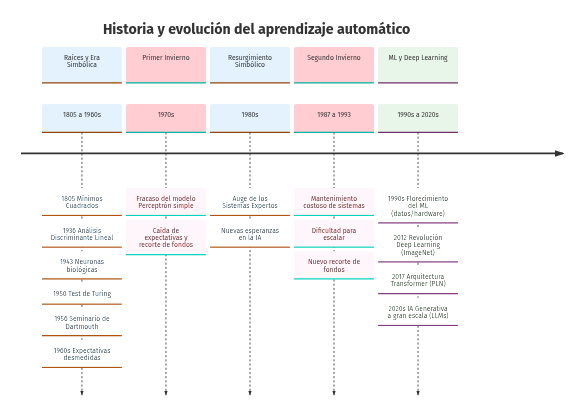
\includegraphics[width=0.62\textwidth]{../book/_static/generated/diagrams_pdf/es/00_fundamentos_01_historia_evolucion_01.png}
  \end{center}
\end{frame}

\begin{frame}{Raíces matemáticas y el Test de Turing (1805-1950)}
  \begin{columns}
    \begin{column}{0.6\textwidth}
      \begin{itemize}
        \item 1805: Legendre y Gauss, \textbf{mínimos cuadrados}
        \item 1936: Fisher, análisis discriminante lineal
        \item 1943: McCulloch y Pitts, primera neurona artificial
        \item 1950: Alan Turing, \textit{``Computing Machinery and Intelligence''} — el \textbf{Test de Turing}
      \end{itemize}
    \end{column}
    \begin{column}{0.35\textwidth}
      \centering
      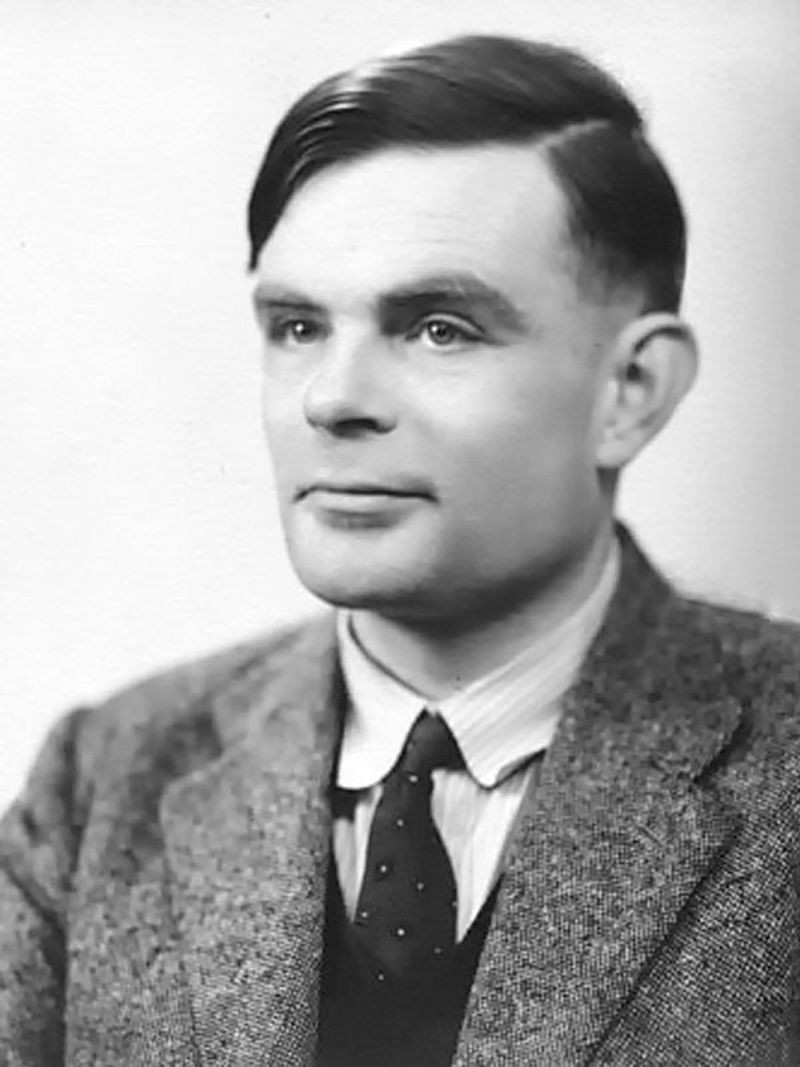
\includegraphics[width=0.85\textwidth]{../book/_static/external_images/alan_turing_1951.jpg}\\[0.3em]
      {\tiny\textit{Fuente: Elliott \& Fry (1951), dominio público}}
    \end{column}
  \end{columns}
\end{frame}

\begin{frame}{El Perceptrón y los inviernos de la IA}
  \begin{columns}
    \begin{column}{0.6\textwidth}
      \begin{itemize}
        \item 1958: Frank Rosenblatt crea el \textbf{Perceptrón}
        \item \textbf{Primer invierno} (años 70): el Perceptrón no resuelve problemas no lineales
        \item 1956: nace formalmente la IA (seminario de Dartmouth)
        \item \textbf{Segundo invierno} (años 90): sistemas expertos caros y poco escalables
      \end{itemize}
    \end{column}
    \begin{column}{0.35\textwidth}
      \centering
      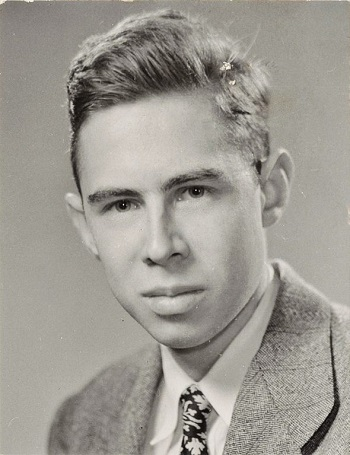
\includegraphics[width=\textwidth]{../book/_static/external_images/frank_rosenblatt.jpg}\\
      \fuente{Heinz Nixdorf MuseumsForum, CC BY-SA 4.0}
    \end{column}
  \end{columns}
\end{frame}

\begin{frame}{Deep Learning y la era de los LLM (2010-hoy)}
  \begin{itemize}
    \item 2012: victoria de Hinton en el desafío \textbf{ImageNet}
    \item \textbf{MNIST}: banco de pruebas clásico para clasificación de dígitos
    \item 2017: arquitectura \textbf{Transformer} — revolución en PLN
    \item 2020s: \textbf{IA Generativa} (ChatGPT, Gemini) a escala de miles de millones de parámetros
  \end{itemize}
  \begin{center}
    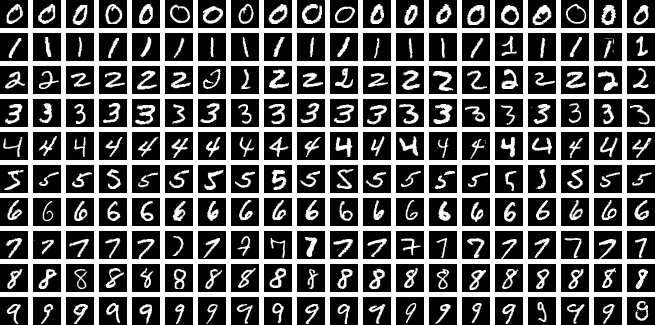
\includegraphics[width=0.55\textwidth]{../book/_static/external_images/mnist_dataset_example.png}\\
    \fuente{Suvanjanprasai (2024), Wikimedia Commons, CC BY-SA 4.0}
  \end{center}
\end{frame}

\subsection{1.2 Conceptos fundamentales}

\begin{frame}{Datos, \textit{features} y etiquetas}
  \begin{center}
    \begin{tabular}{lcccc}
      \toprule
      Muestra & Feature 1 & Feature 2 & Feature 3 & Label \\
      \midrule
      1 & 25 & 70 & 175 & Gato \\
      2 & 8 & 4 & 90 & Gato \\
      3 & 35 & 80 & 180 & Perro \\
      \bottomrule
    \end{tabular}
  \end{center}
  \vspace{1em}
  \begin{itemize}
    \item \textbf{Muestra}: punto de datos individual
    \item \textbf{Features}: atributos que describen la muestra
    \item \textbf{Etiqueta (label)}: lo que queremos predecir — la ``verdad fundamental''
  \end{itemize}
\end{frame}

\begin{frame}{Overfitting vs. underfitting}
  \begin{itemize}
    \item \textbf{Underfitting}: el modelo es demasiado simple, no capta el patrón (alto sesgo)
    \item \textbf{Overfitting}: el modelo memoriza el ruido de entrenamiento (alta varianza)
    \item Objetivo: el equilibrio sesgo-varianza que mejor generaliza
  \end{itemize}
  \begin{center}
    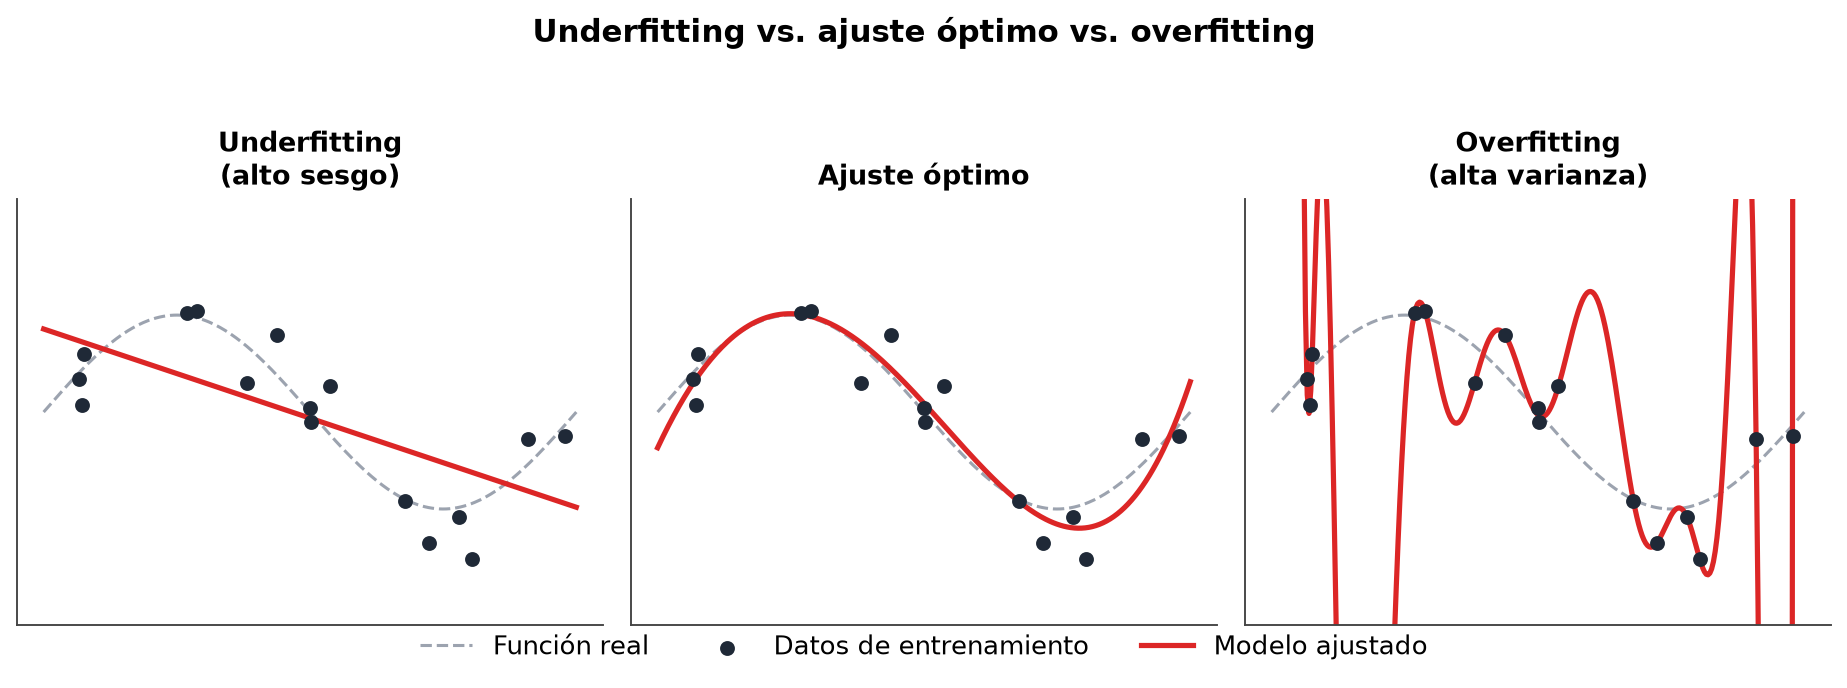
\includegraphics[width=0.75\textwidth]{../book/_static/generated/figures/es/overfitting_underfitting.png}
  \end{center}
\end{frame}

\begin{frame}{Validación cruzada $K$-fold}
  \begin{itemize}
    \item Divide los datos en $K$ particiones (\textit{folds}); cada una actúa una vez como test
    \item Métrica final = media de los $K$ resultados $\rightarrow$ estimación más robusta
    \item Evita depender de una única partición train/test
  \end{itemize}
  \begin{center}
    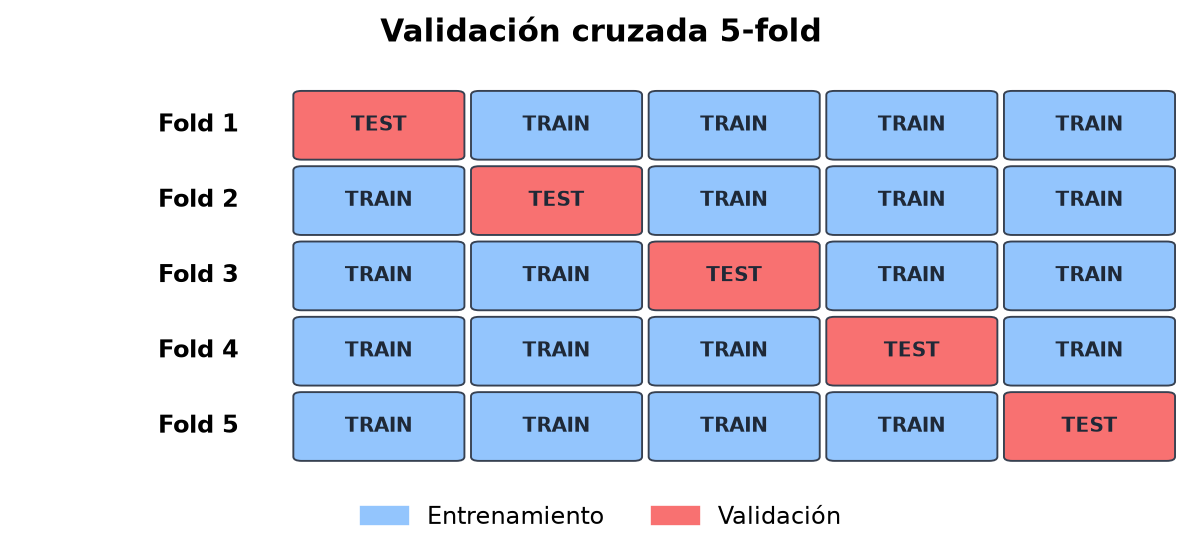
\includegraphics[width=0.62\textwidth]{../book/_static/generated/figures/es/kfold_cross_validation.png}
  \end{center}
\end{frame}

\begin{frame}{Matriz de confusión y métricas}
  \begin{columns}
    \begin{column}{0.5\textwidth}
      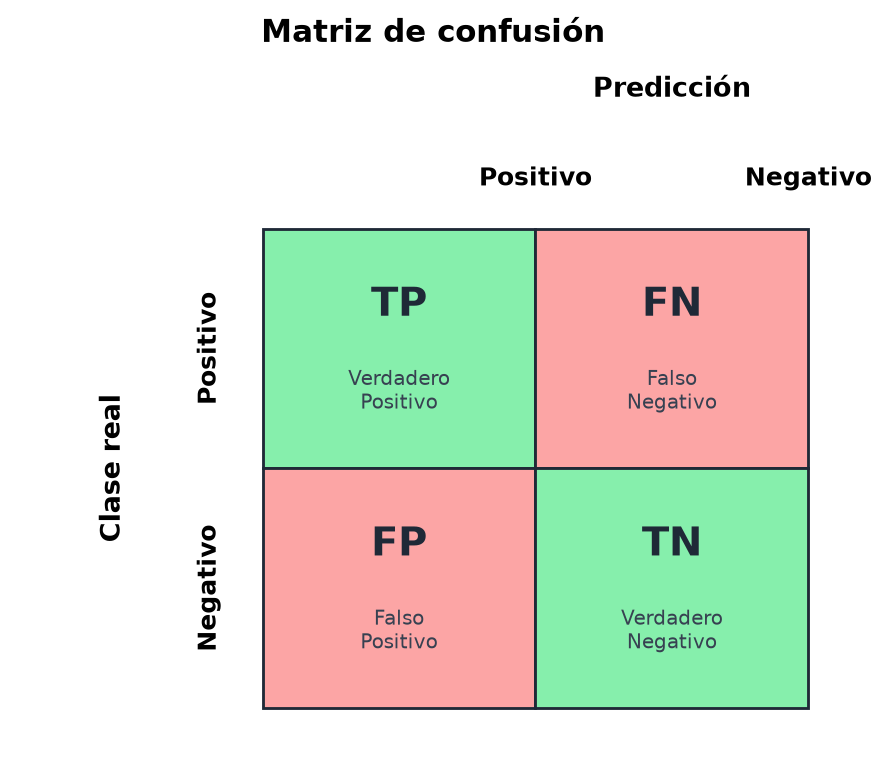
\includegraphics[width=\textwidth]{../book/_static/generated/figures/es/confusion_matrix.png}
    \end{column}
    \begin{column}{0.5\textwidth}
      \small
      \begin{align*}
        \text{Precisión} &= \frac{TP}{TP+FP} \\
        \text{Recall} &= \frac{TP}{TP+FN} \\
        F1 &= 2\cdot\frac{P \times R}{P + R}
      \end{align*}
    \end{column}
  \end{columns}
  \vspace{0.5em}
  \footnotesize
  TP/TN: aciertos; FP/FN: errores. El F1 equilibra precisión y recall, útil con clases desbalanceadas.
\end{frame}

\begin{frame}{El \textit{pipeline} de ML: 10 etapas}
  \begin{columns}
    \begin{column}{0.42\textwidth}
      \footnotesize
      \begin{itemize}
        \item Proceso \textbf{iterativo}: la evaluación puede obligar a volver a etapas anteriores
        \item Gran parte del esfuerzo real está en las etapas 2-3 (datos) y 7-8 (ajuste)
        \item El despliegue no es el final: requiere monitorización continua
      \end{itemize}
    \end{column}
    \begin{column}{0.55\textwidth}
      \centering
      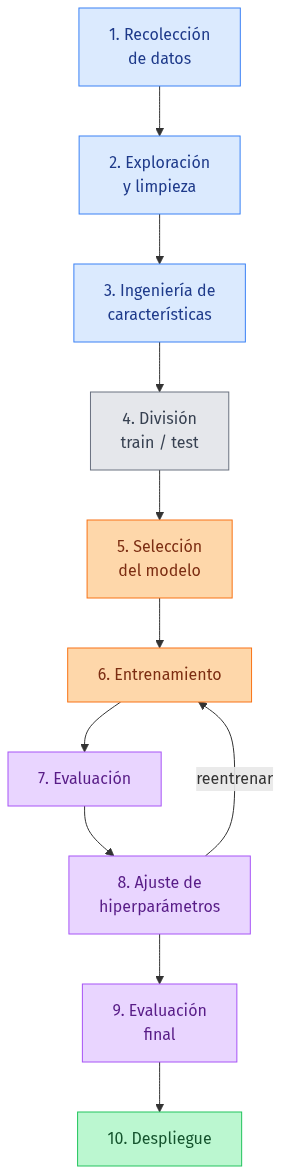
\includegraphics[height=0.8\textheight]{../book/_static/generated/diagrams_pdf/es/00_fundamentos_02_conceptos_fundamentales_01.png}
    \end{column}
  \end{columns}
\end{frame}

% ============================================================
\section{Aprendizaje Supervisado}
\begin{frame}
  \centering
  {\Huge Sección 2}\\[0.5em]
  {\Large Aprendizaje Supervisado}
\end{frame}

\subsection{2.1 Regresión}

\begin{frame}{Regresión lineal}
  \begin{itemize}
    \item Predice un \textbf{valor continuo} $Y$ a partir de predictores $X$
    \item Simple: $Y \approx \beta_0 + \beta_1 X$
    \item Múltiple: $Y = \beta_0 + \beta_1X_1 + \dots + \beta_pX_p + \epsilon$
    \item \textbf{OLS}: minimiza la suma de residuos al cuadrado (RSS)
  \end{itemize}
\end{frame}

\begin{frame}{Ejemplo real: dataset \textit{Advertising}}
  \begin{itemize}
    \item Predice las ventas (\textit{Sales}) a partir de la inversión en TV, radio y prensa
    \item La recta minimiza la suma de residuos al cuadrado (OLS)
    \item Ejemplo clásico de regresión lineal simple
  \end{itemize}
  \begin{center}
    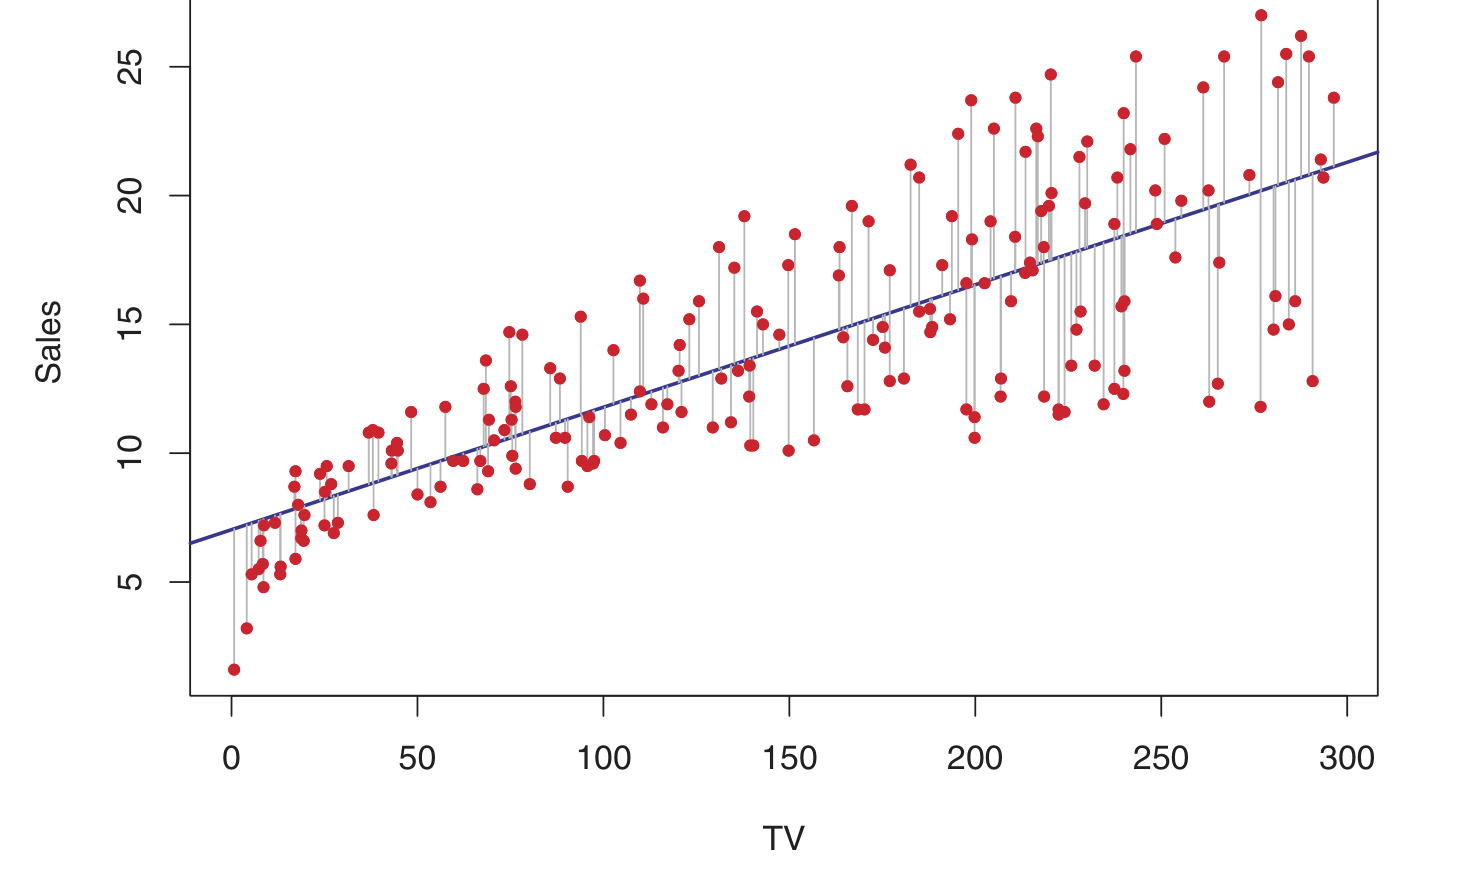
\includegraphics[width=0.48\textwidth]{../book/_static/book_figures/islr_fig3_1_advertising.png}
  \end{center}
  \fuente{James, Witten, Hastie \& Tibshirani (2013), \textit{An Introduction to Statistical Learning}, Fig. 3.1. Libro de libre distribución (statlearning.com).}
\end{frame}

\begin{frame}{Descenso de gradiente}
  \begin{itemize}
    \item Algoritmo iterativo: actualiza los parámetros en la dirección opuesta al gradiente
    \item $\theta \leftarrow \theta - \alpha \nabla J(\theta)$, donde $\alpha$ es la tasa de aprendizaje
    \item Una tasa muy alta diverge; una muy baja converge lentamente
  \end{itemize}
  \begin{center}
    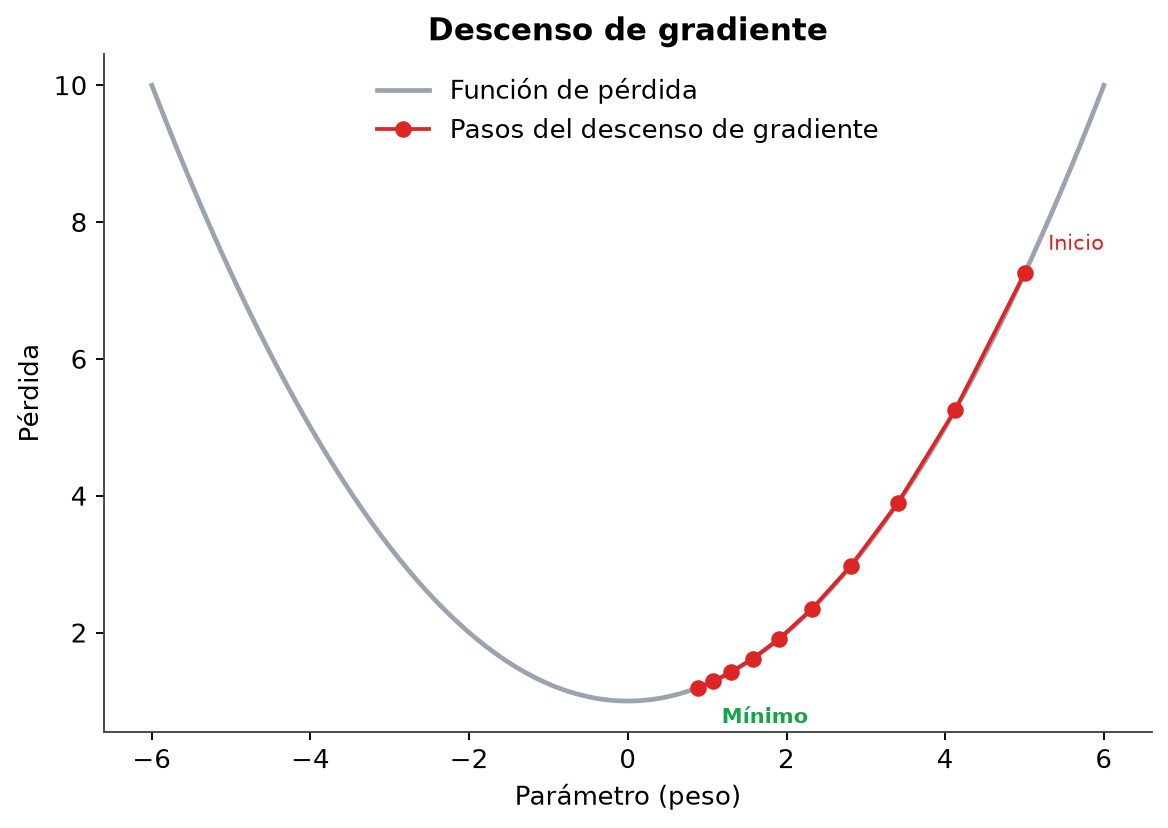
\includegraphics[width=0.5\textwidth]{../book/_static/generated/figures/es/gradient_descent.png}
  \end{center}
\end{frame}

\begin{frame}{Regularización: Ridge y Lasso}
  \begin{itemize}
    \item \textbf{Ridge} ($L_2$): penaliza $\sum \beta_j^2$, encoge los coeficientes sin anularlos
    \item \textbf{Lasso} ($L_1$): penaliza $\sum |\beta_j|$, puede anular coeficientes (selección de variables)
    \item $\lambda$ controla la fuerza de la penalización
  \end{itemize}
  \begin{center}
    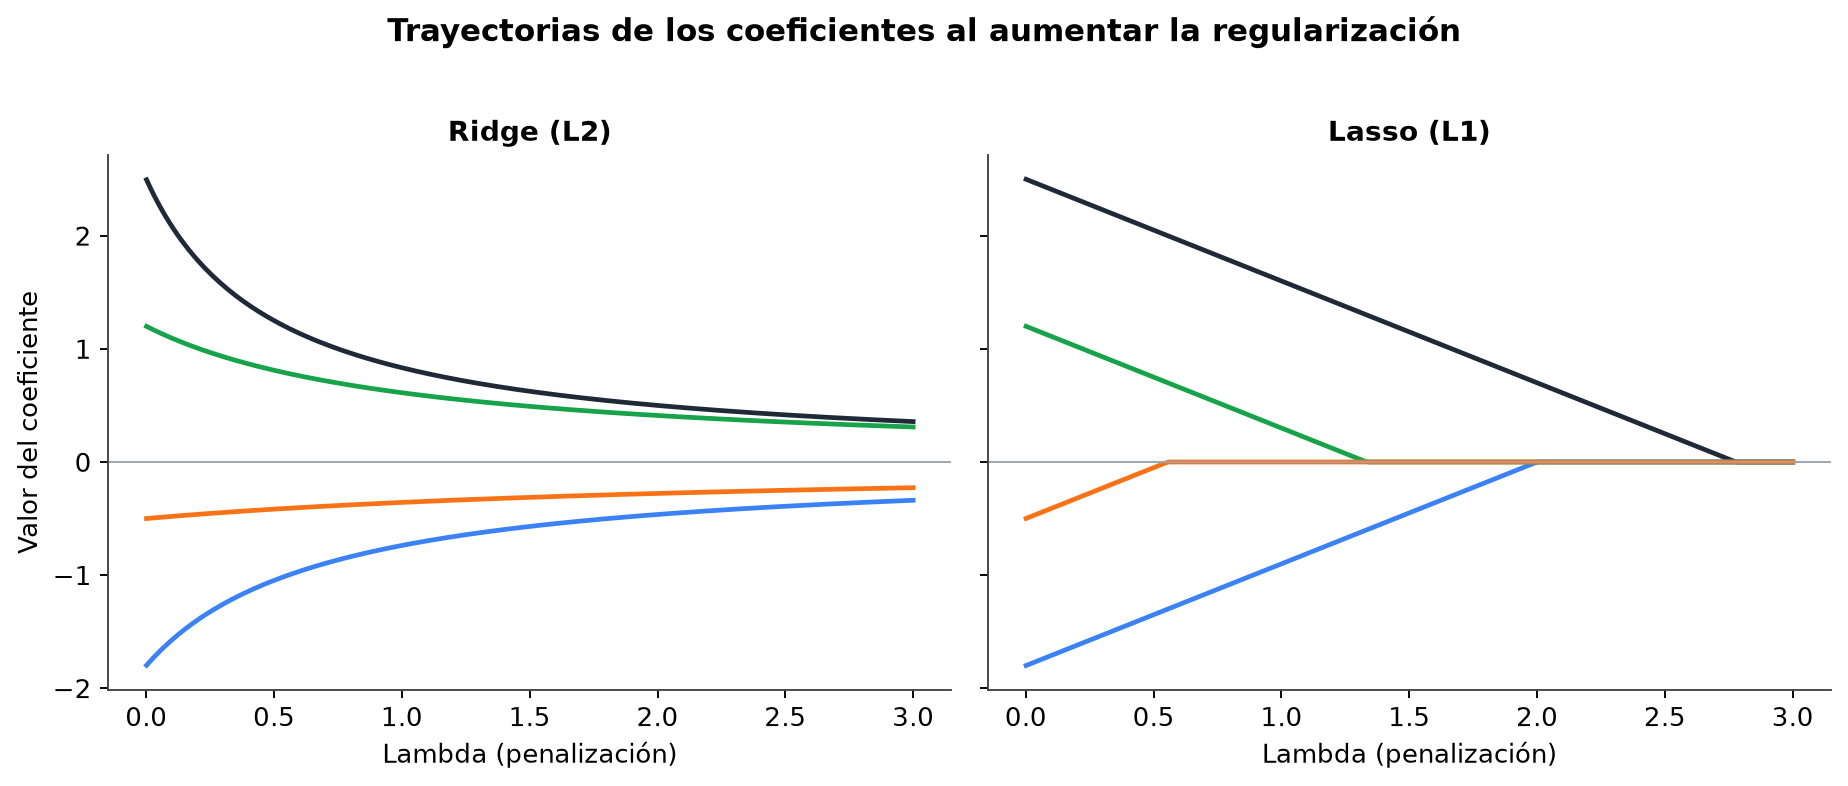
\includegraphics[width=0.7\textwidth]{../book/_static/generated/figures/es/regularization_paths.png}
  \end{center}
\end{frame}

\begin{frame}{Ridge en datos reales: dataset \textit{Credit}}
  \begin{itemize}
    \item Al aumentar $\lambda$, los coeficientes se encogen hacia cero
    \item Reduce la varianza a cambio de un pequeño aumento del sesgo
  \end{itemize}
  \begin{center}
    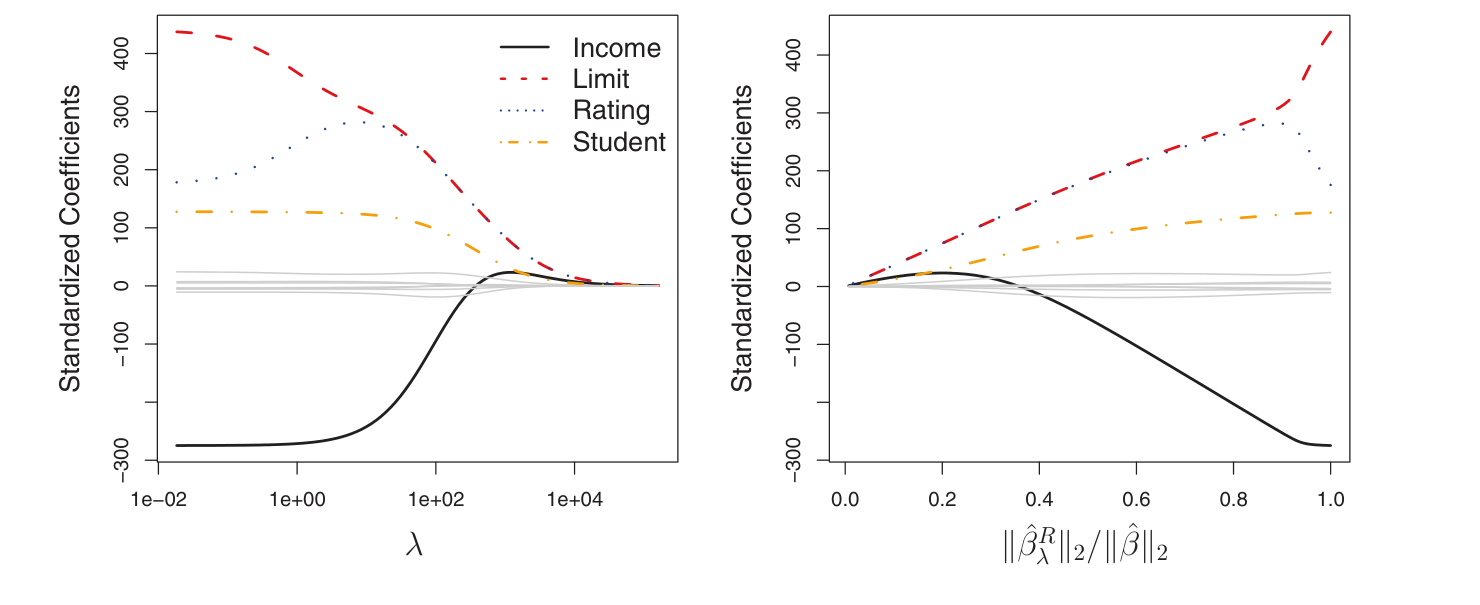
\includegraphics[width=0.65\textwidth]{../book/_static/book_figures/islr_fig6_4_ridge_credit.png}
  \end{center}
  \fuente{James, Witten, Hastie \& Tibshirani (2013), \textit{An Introduction to Statistical Learning}, Fig. 6.4.}
\end{frame}

\subsection{2.2 Clasificación}

\begin{frame}{La función sigmoide}
  \begin{itemize}
    \item Transforma cualquier valor real en una probabilidad entre 0 y 1
    \item $\sigma(z) = \dfrac{1}{1+e^{-z}}$
    \item Es la base de la regresión logística
  \end{itemize}
  \begin{center}
    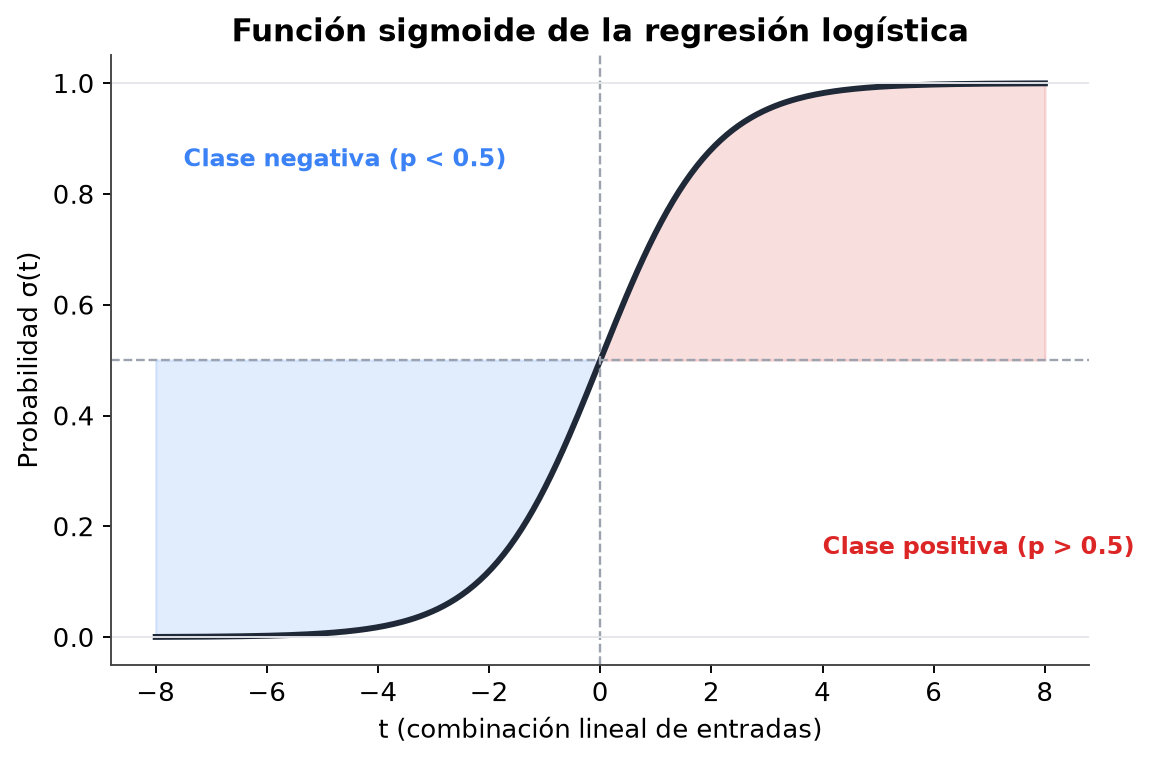
\includegraphics[width=0.5\textwidth]{../book/_static/generated/figures/es/sigmoid_function.png}
  \end{center}
\end{frame}

\begin{frame}{¿Por qué no usar regresión lineal?}
  \begin{itemize}
    \item La regresión lineal puede predecir probabilidades $<0$ o $>1$ (sin sentido)
    \item La regresión logística usa la sigmoide para mantener la salida en $[0,1]$
  \end{itemize}
  \begin{center}
    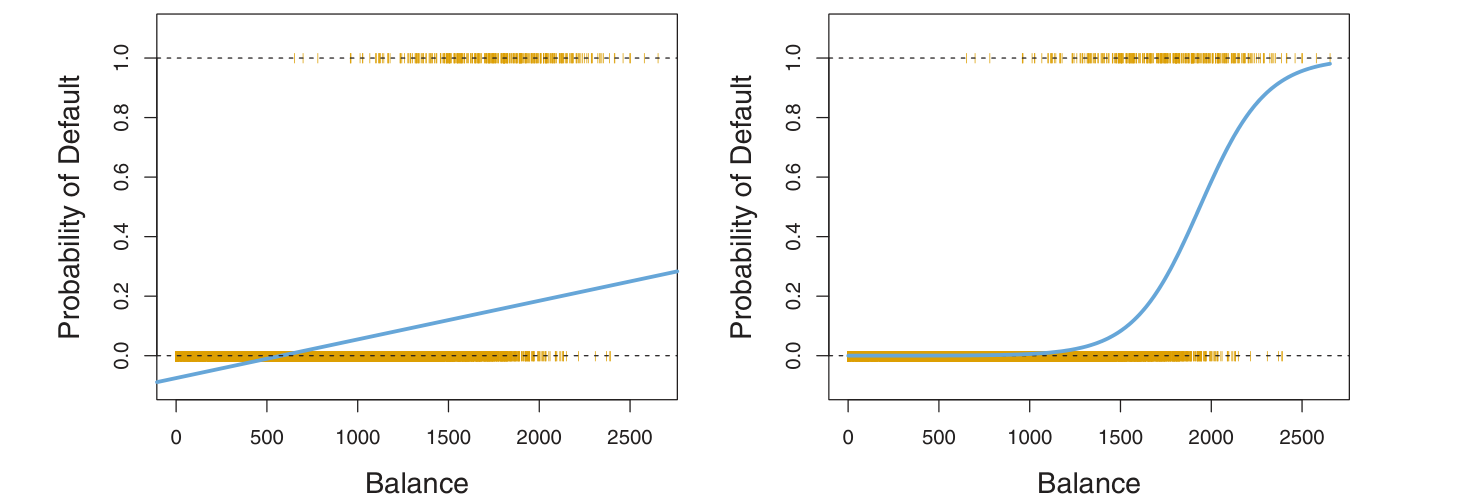
\includegraphics[width=0.7\textwidth]{../book/_static/book_figures/islr_fig4_2_default_logistic.png}
  \end{center}
  \fuente{James, Witten, Hastie \& Tibshirani (2013), \textit{An Introduction to Statistical Learning}, Fig. 4.2.}
\end{frame}

\begin{frame}{Árboles de decisión}
  \begin{columns}
    \begin{column}{0.45\textwidth}
      \begin{itemize}
        \item Divide el espacio de \textit{features} con cortes ortogonales sucesivos
        \item Cada división minimiza la impureza (Gini o entropía) de los nodos hijos
        \item Fáciles de interpretar, pero propensos a overfitting sin poda
      \end{itemize}
    \end{column}
    \begin{column}{0.5\textwidth}
      \centering
      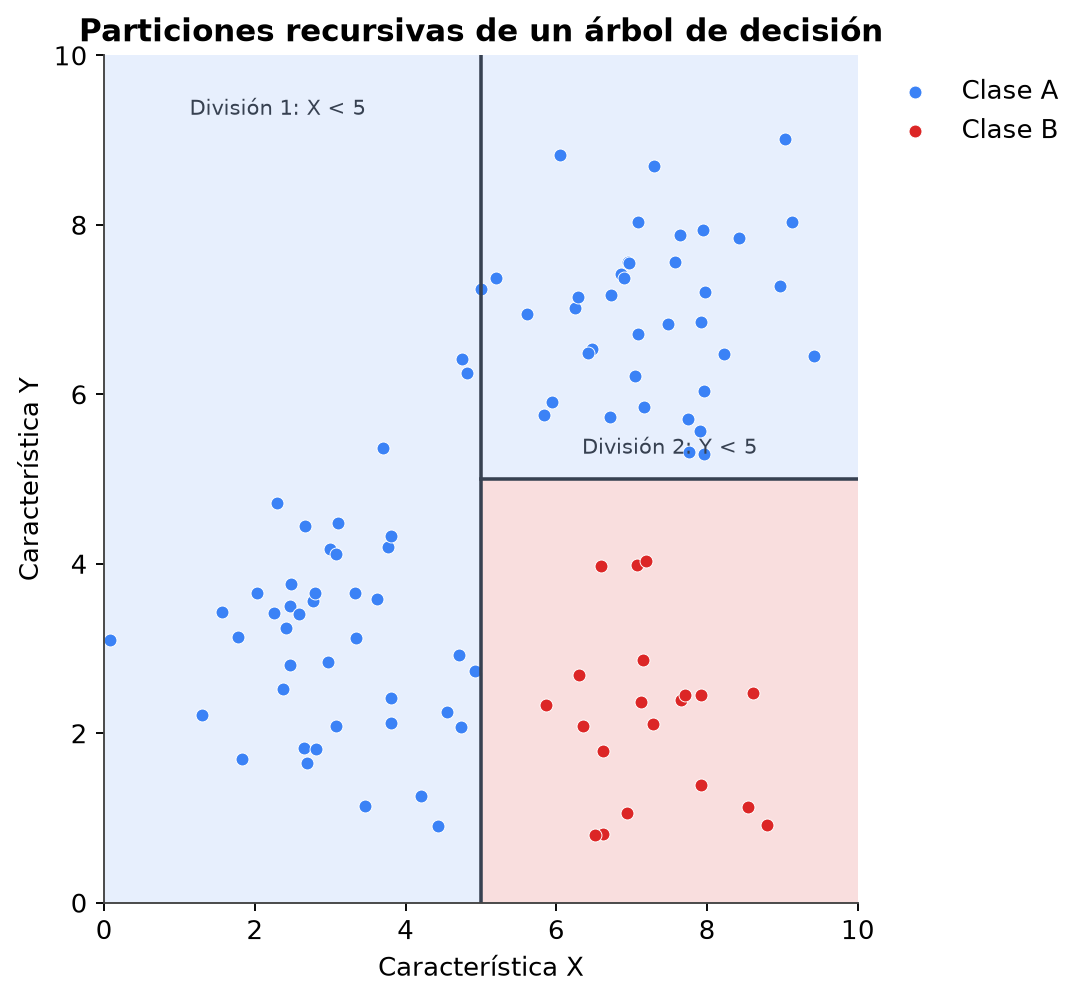
\includegraphics[width=\textwidth]{../book/_static/generated/figures/es/decision_tree_partition.png}
    \end{column}
  \end{columns}
\end{frame}

\begin{frame}{Ensembles: Random Forest y Boosting}
  \begin{itemize}
    \item \textbf{Random Forest}: \textit{bagging} + subconjunto aleatorio de features en cada división
    \item \textbf{Boosting}: modelos secuenciales que corrigen los errores del anterior (XGBoost, LightGBM)
    \item \textbf{Voting / Stacking}: combinan las salidas de varios modelos independientes
  \end{itemize}
\end{frame}

\begin{frame}{SVM: margen máximo}
  \begin{columns}
    \begin{column}{0.45\textwidth}
      \begin{itemize}
        \item Busca el hiperplano que maximiza el margen entre clases
        \item Los vectores de soporte son los puntos más cercanos al hiperplano
        \item El \textit{kernel trick} permite fronteras no lineales
      \end{itemize}
    \end{column}
    \begin{column}{0.5\textwidth}
      \centering
      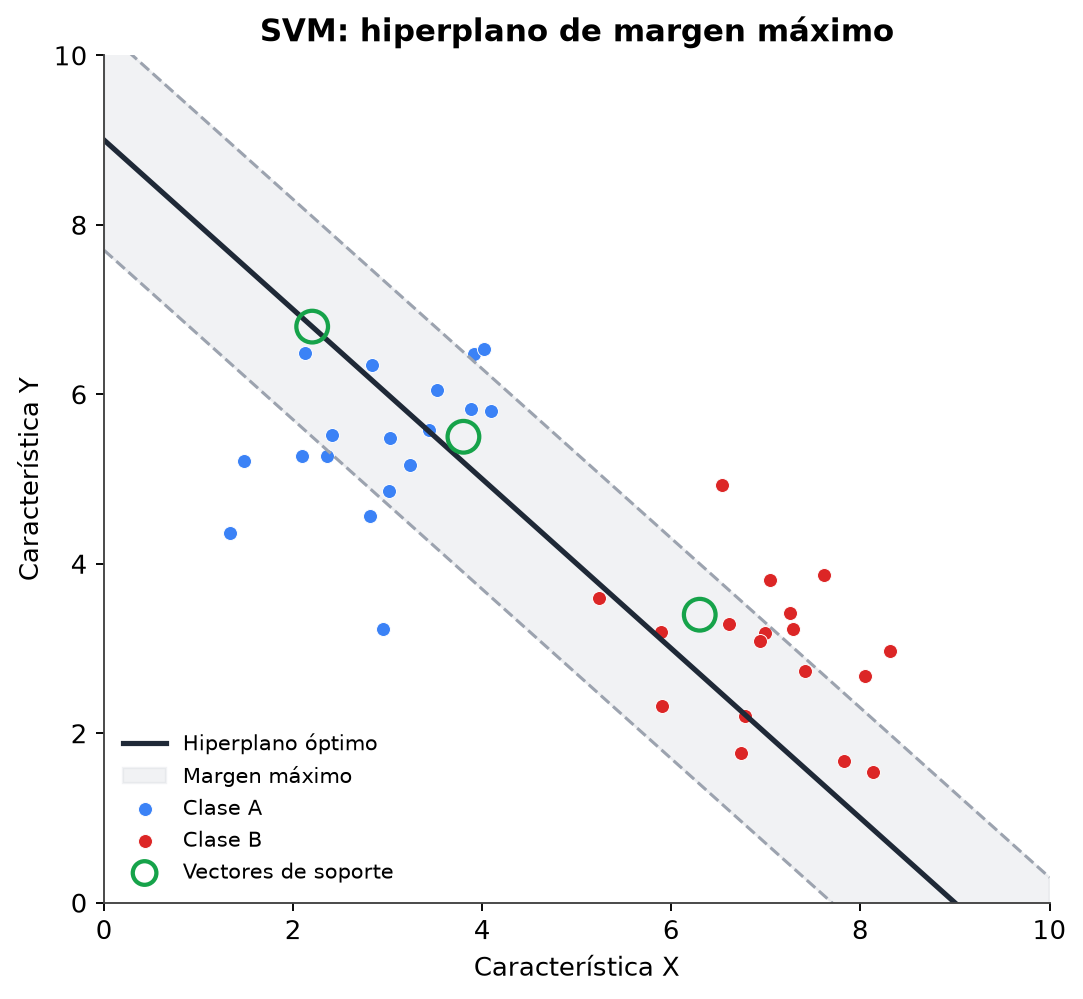
\includegraphics[width=\textwidth]{../book/_static/generated/figures/es/svm_margin.png}
    \end{column}
  \end{columns}
\end{frame}

\begin{frame}{Redes neuronales}
  \begin{itemize}
    \item Capas de neuronas conectadas por pesos ajustables
    \item Cada neurona aplica una función de activación no lineal (ReLU, sigmoide...)
    \item Entrenadas mediante retropropagación (\textit{backpropagation}) del error
  \end{itemize}
  \begin{center}
    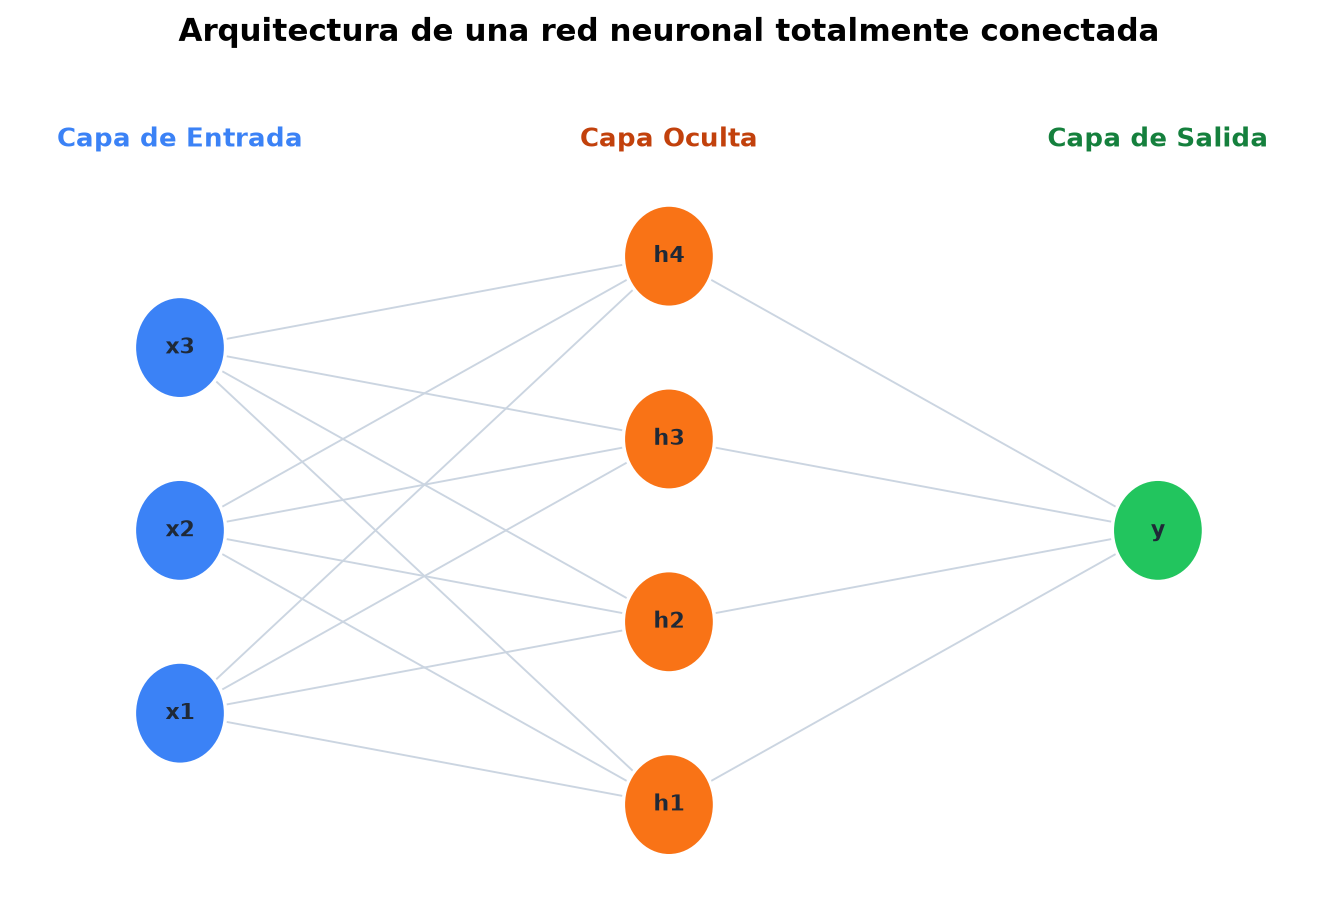
\includegraphics[width=0.5\textwidth]{../book/_static/generated/figures/es/nn_architecture.png}
  \end{center}
\end{frame}

\begin{frame}{Evaluación: curva ROC y AUC}
  \begin{columns}
    \begin{column}{0.45\textwidth}
      \begin{itemize}
        \item Eje Y: tasa de verdaderos positivos; eje X: tasa de falsos positivos
        \item AUC = 1: clasificador perfecto; AUC = 0.5: equivale al azar
        \item Compara modelos sin depender del umbral elegido
      \end{itemize}
    \end{column}
    \begin{column}{0.45\textwidth}
      \centering
      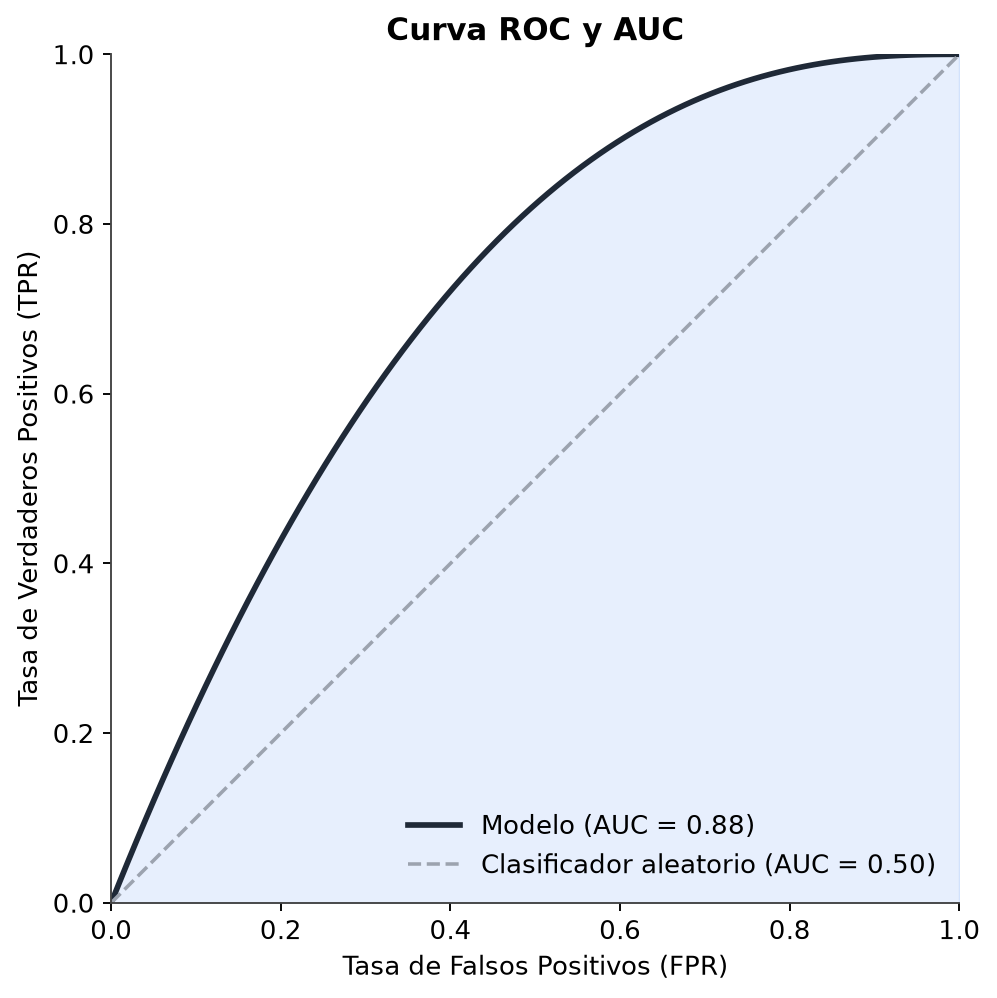
\includegraphics[width=0.9\textwidth]{../book/_static/generated/figures/es/roc_curve.png}
    \end{column}
  \end{columns}
\end{frame}

% ============================================================
\section{Aprendizaje No Supervisado}
\begin{frame}
  \centering
  {\Huge Sección 3}\\[0.5em]
  {\Large Aprendizaje No Supervisado}
\end{frame}

\subsection{3.1 Clustering}

\begin{frame}{¿Qué es el clustering?}
  \begin{itemize}
    \item Sin etiquetas: solo tenemos $X$, sin $y$
    \item Objetivo: agrupar datos con \textbf{alta similitud interna} y \textbf{alta diferenciación externa}
    \item Algoritmos: $K$-means, jerárquico, DBSCAN
  \end{itemize}
\end{frame}

\begin{frame}{Proceso iterativo de $K$-means}
  \footnotesize
  \begin{enumerate}
    \item Inicializa $K$ centroides al azar
    \item Asigna cada punto al centroide más cercano
    \item Recalcula centroides como la media de su cluster; repite hasta converger
  \end{enumerate}
  \begin{center}
    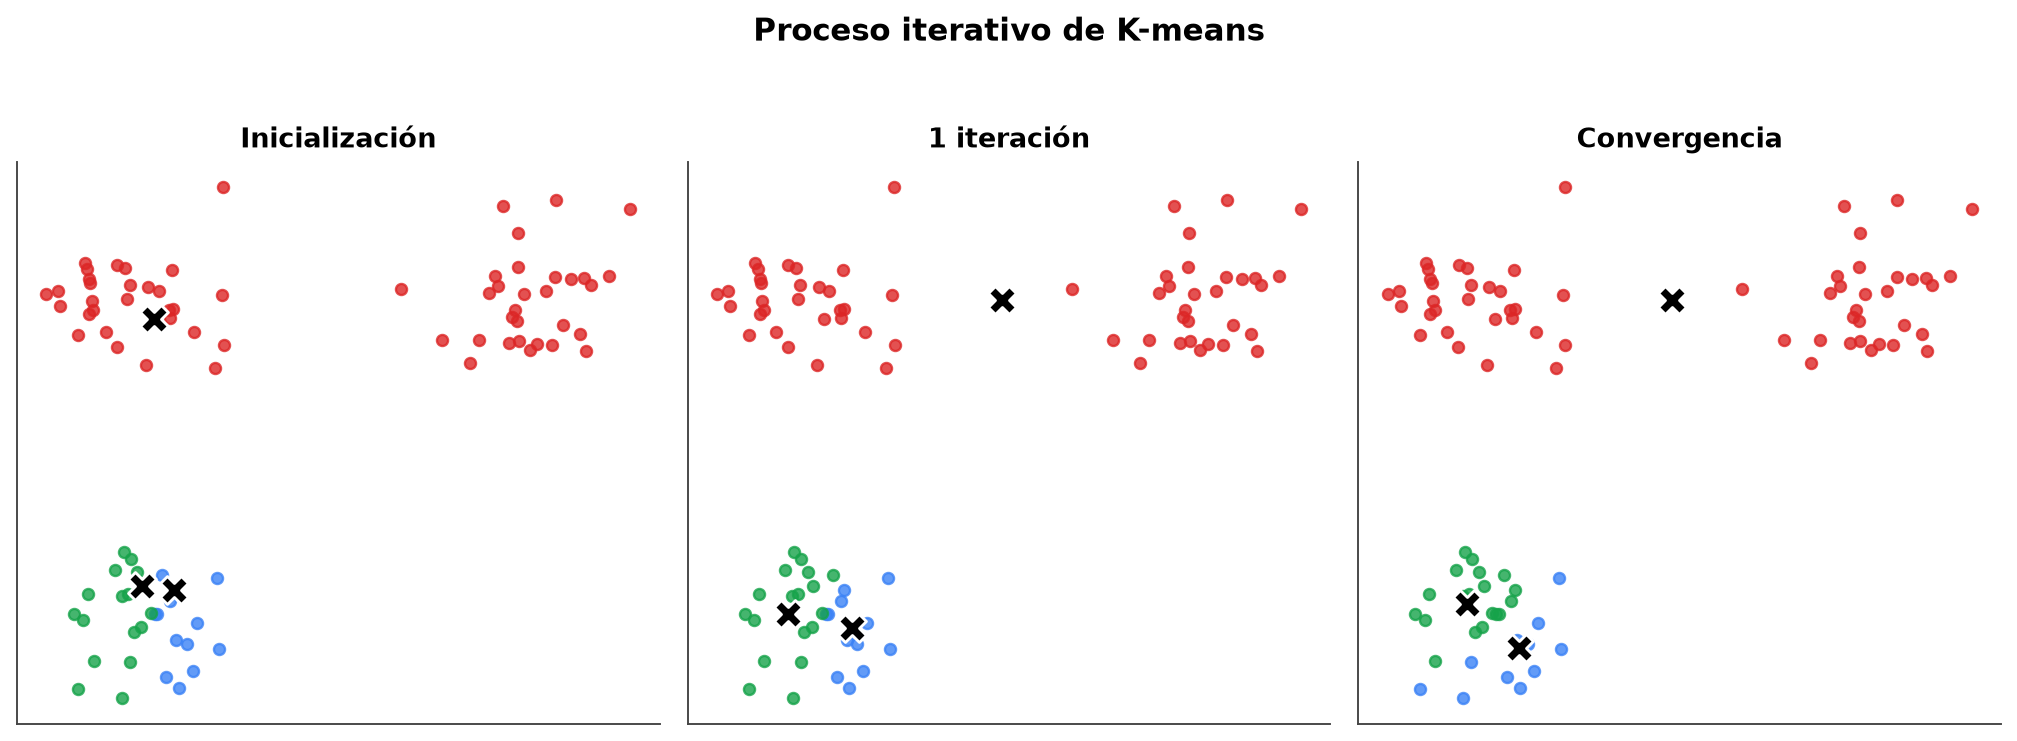
\includegraphics[width=0.85\textwidth]{../book/_static/generated/figures/es/kmeans_process.png}
  \end{center}
\end{frame}

\begin{frame}{Método del codo}
  \begin{itemize}
    \item Representa la inercia (suma de distancias al cuadrado) frente a $K$
    \item El ``codo'' señala el punto de rendimientos decrecientes: el $K$ óptimo
  \end{itemize}
  \begin{center}
    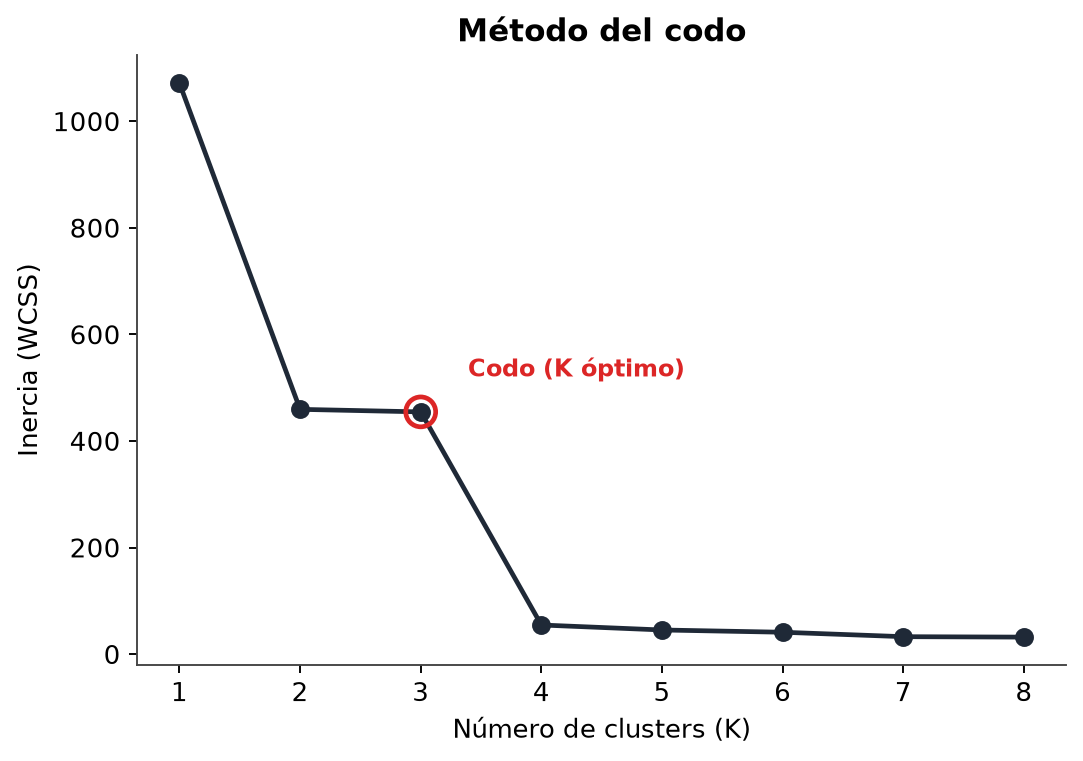
\includegraphics[width=0.5\textwidth]{../book/_static/generated/figures/es/elbow_method.png}
  \end{center}
\end{frame}

\begin{frame}{Clustering jerárquico: dendrograma}
  \begin{itemize}
    \item Construye una jerarquía de clusters sin fijar $K$ de antemano
    \item Cortar el dendrograma a una altura dada define el número de clusters
  \end{itemize}
  \begin{center}
    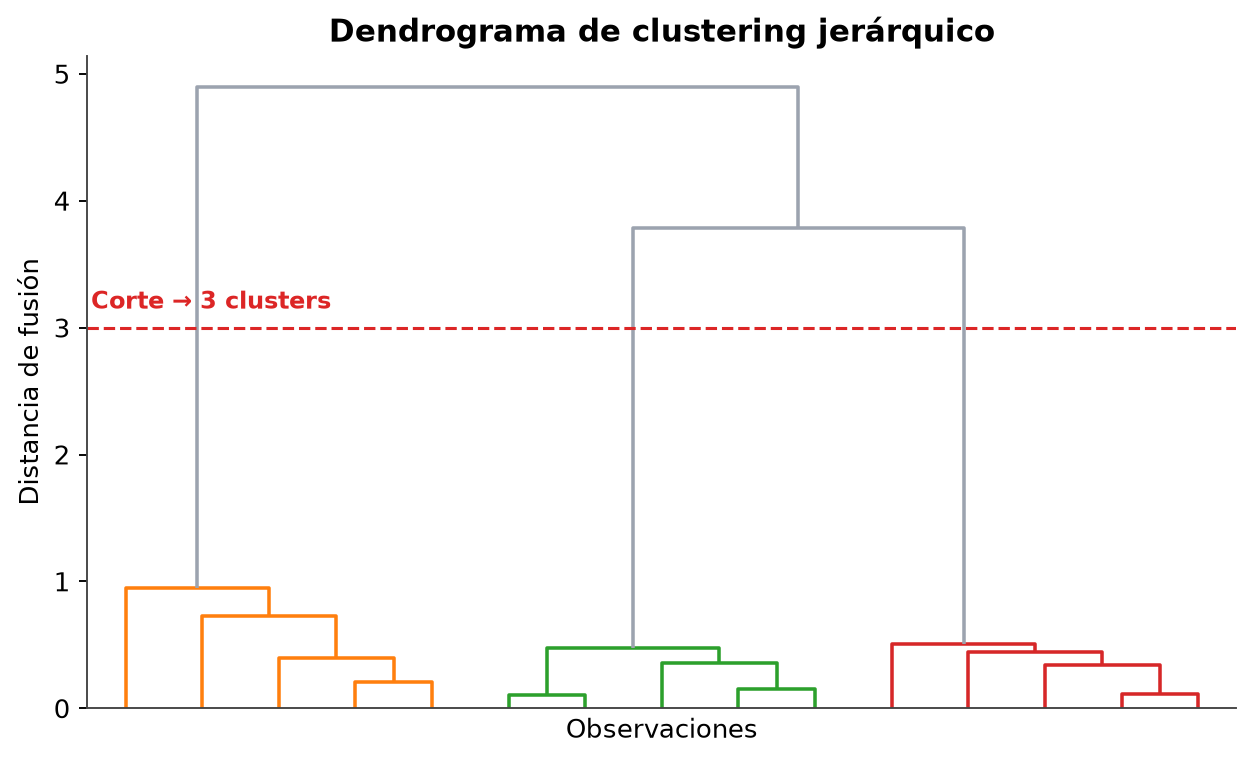
\includegraphics[width=0.6\textwidth]{../book/_static/generated/figures/es/dendrogram.png}
  \end{center}
\end{frame}

\begin{frame}{Datos reales: NCI60 (líneas celulares de cáncer)}
  \begin{columns}
    \begin{column}{0.45\textwidth}
      \begin{itemize}
        \item Agrupa líneas celulares de cáncer por similitud de expresión génica
        \item Líneas del mismo tipo de cáncer tienden a agruparse en la misma rama
      \end{itemize}
      \fuente{James, Witten, Hastie \& Tibshirani (2013), \textit{An Introduction to Statistical Learning}, Fig. 10.17.}
    \end{column}
    \begin{column}{0.4\textwidth}
      \centering
      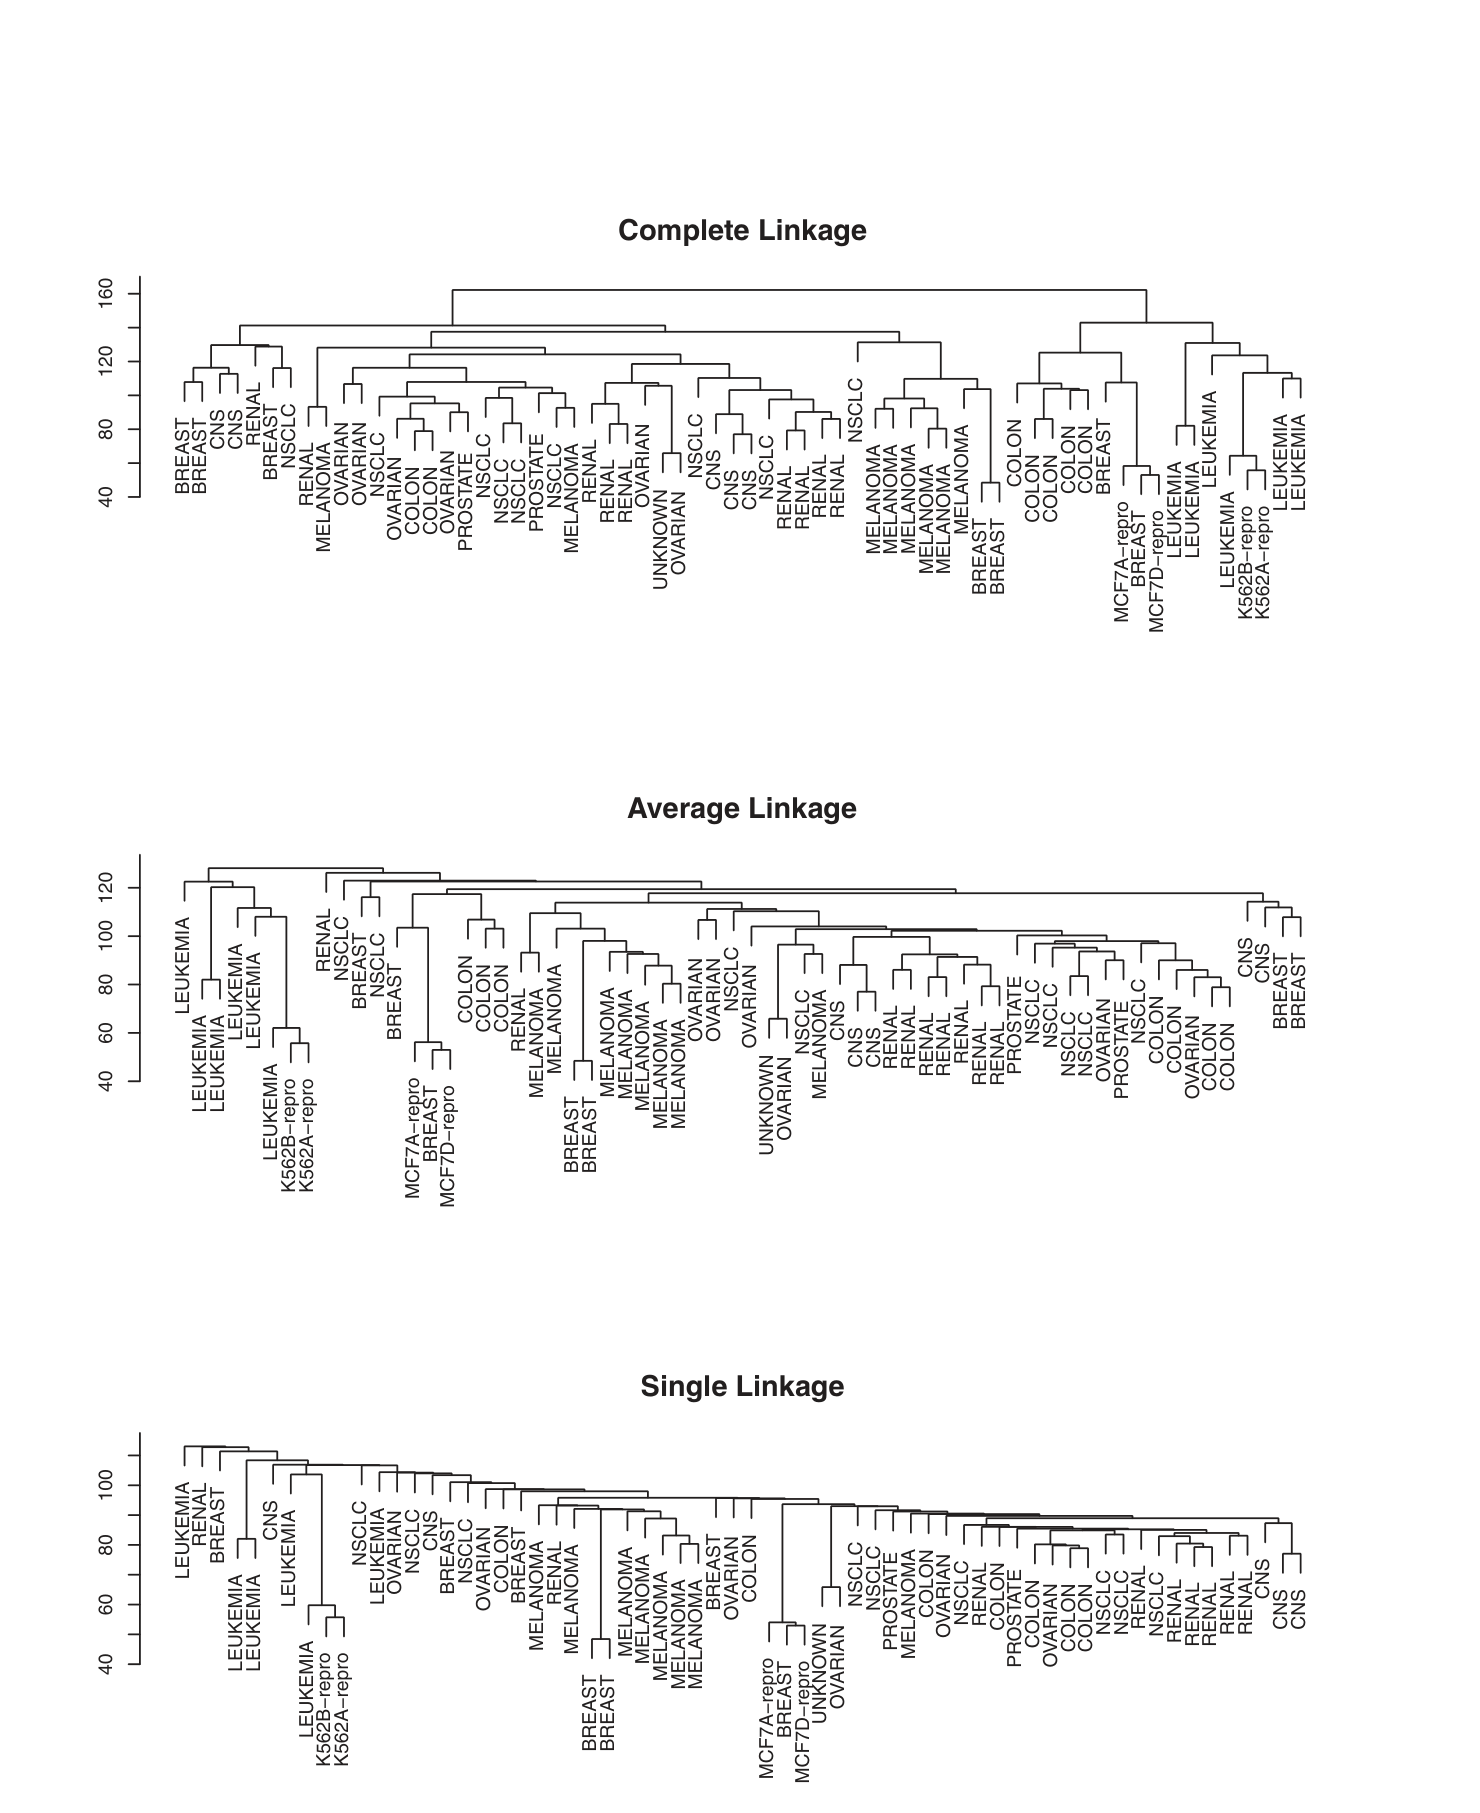
\includegraphics[width=\textwidth]{../book/_static/book_figures/islr_fig10_17_nci60_dendrogram.png}
    \end{column}
  \end{columns}
\end{frame}

\begin{frame}{DBSCAN vs. $K$-means}
  \footnotesize
  DBSCAN agrupa por densidad: no necesita fijar $K$, detecta formas arbitrarias e identifica automáticamente el ruido (puntos que no pertenecen a ningún cluster).
  \begin{center}
    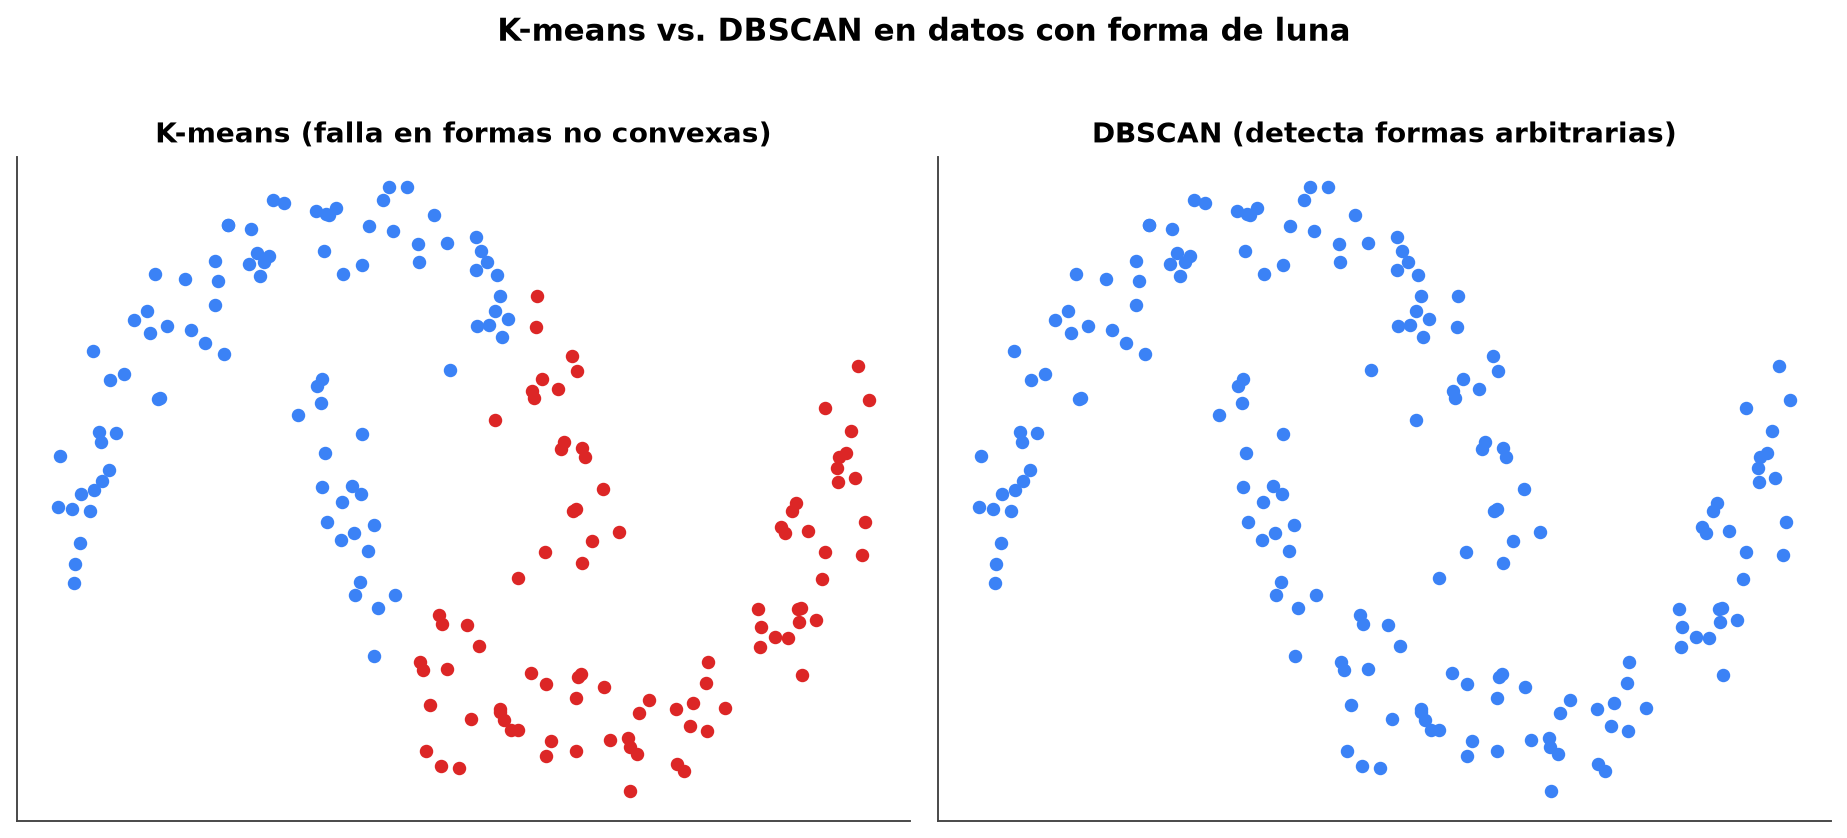
\includegraphics[width=0.85\textwidth]{../book/_static/generated/figures/es/dbscan_vs_kmeans.png}
  \end{center}
\end{frame}

\begin{frame}{Evaluación: coeficiente de silueta}
  \begin{itemize}
    \item Mide cuán similar es un punto a su propio cluster frente a los demás
    \item Rango $[-1, 1]$: valores altos indican clusters bien separados
  \end{itemize}
  \begin{center}
    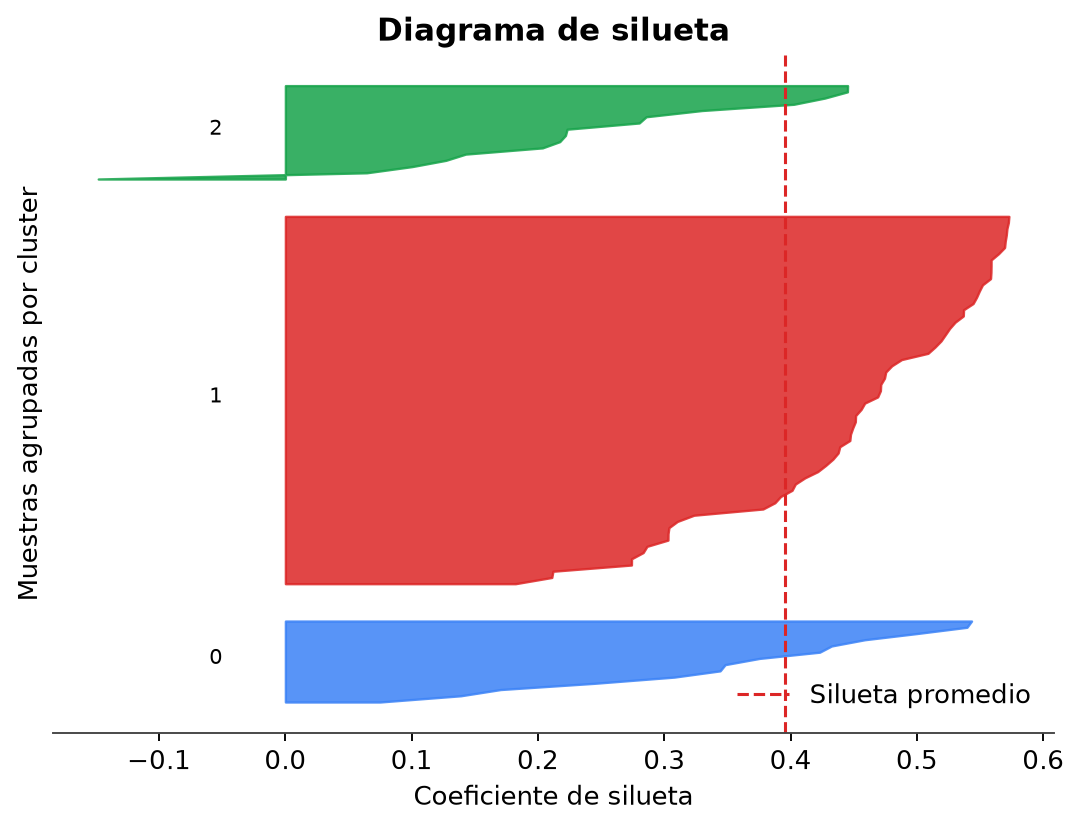
\includegraphics[width=0.45\textwidth]{../book/_static/generated/figures/es/silhouette_diagram.png}
  \end{center}
\end{frame}

\subsection{3.2 Reducción de dimensionalidad}

\begin{frame}{La maldición de la dimensionalidad}
  \footnotesize
  Al aumentar las dimensiones, los datos se vuelven extremadamente dispersos y las distancias entre puntos se vuelven casi indistinguibles.
  \begin{center}
    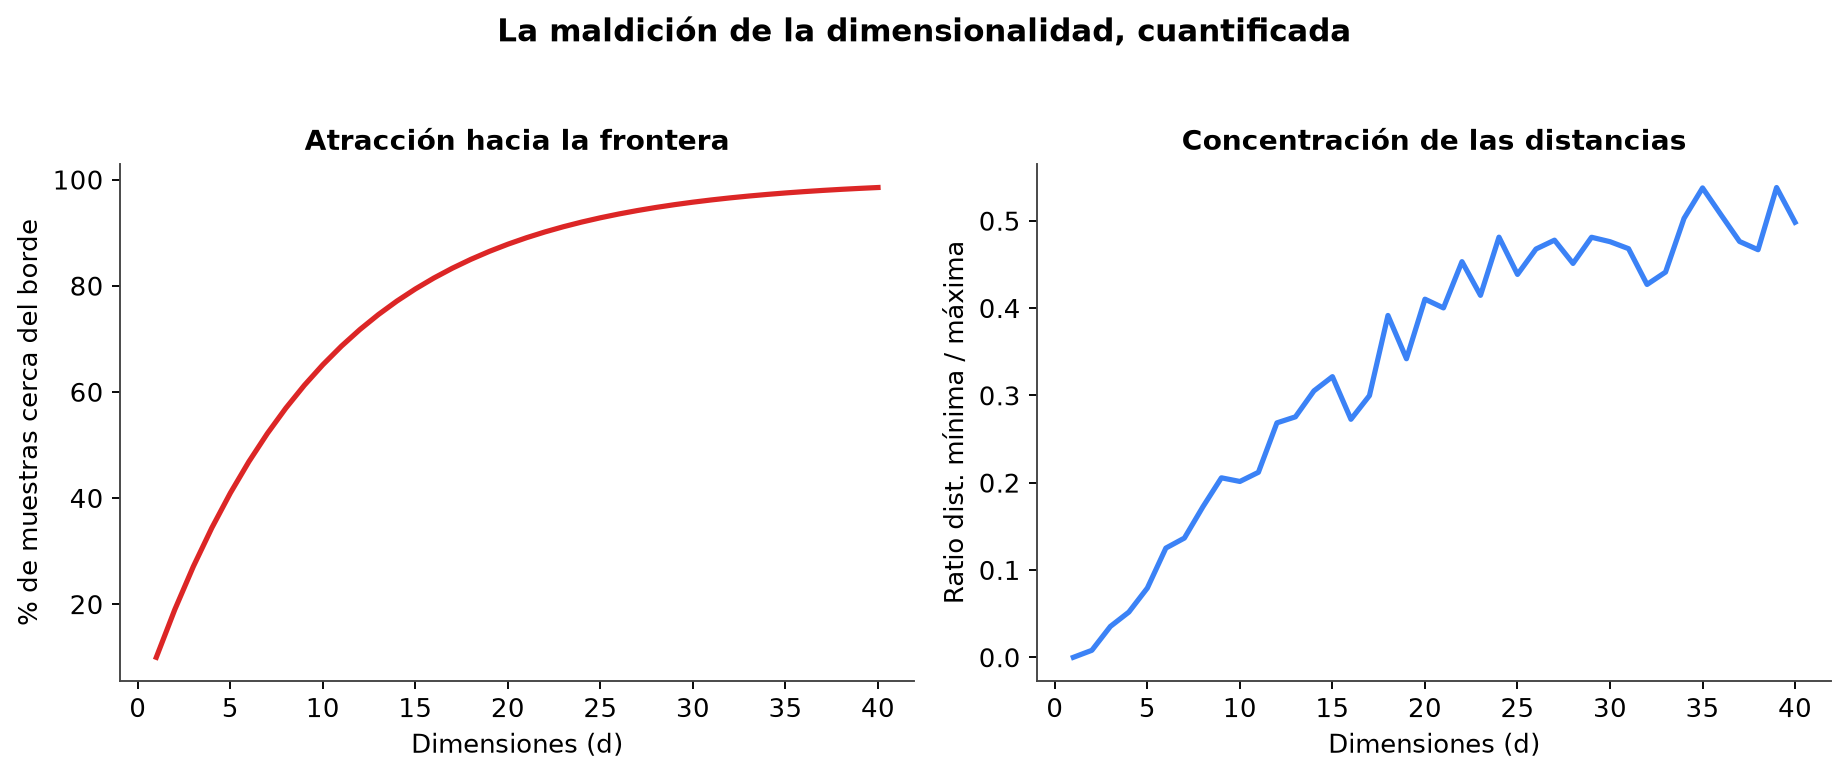
\includegraphics[width=0.85\textwidth]{../book/_static/generated/figures/es/curse_of_dimensionality.png}
  \end{center}
\end{frame}

\begin{frame}{PCA: componentes principales}
  \begin{itemize}
    \item PC1: dirección de máxima varianza; PC2: ortogonal a PC1, máxima varianza restante
    \item Reduce dimensiones conservando la mayor parte de la información
  \end{itemize}
  \begin{center}
    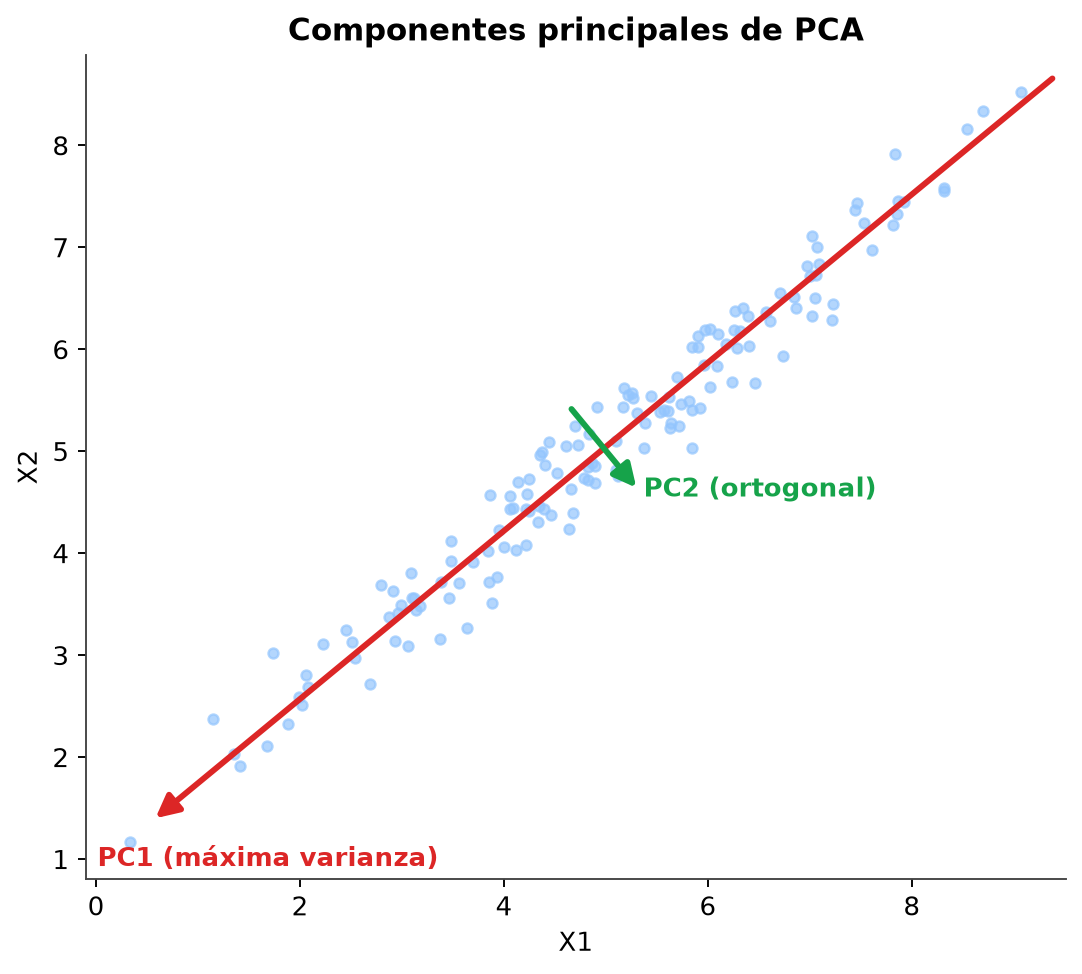
\includegraphics[width=0.45\textwidth]{../book/_static/generated/figures/es/pca_projection.png}
  \end{center}
\end{frame}

\begin{frame}{PCA en datos reales: NCI60 (6830 genes)}
  \footnotesize
  De 6830 genes a solo 3 componentes principales: las líneas del mismo tipo de cáncer (mismo color) se agrupan a pesar de la enorme dimensionalidad original.
  \begin{center}
    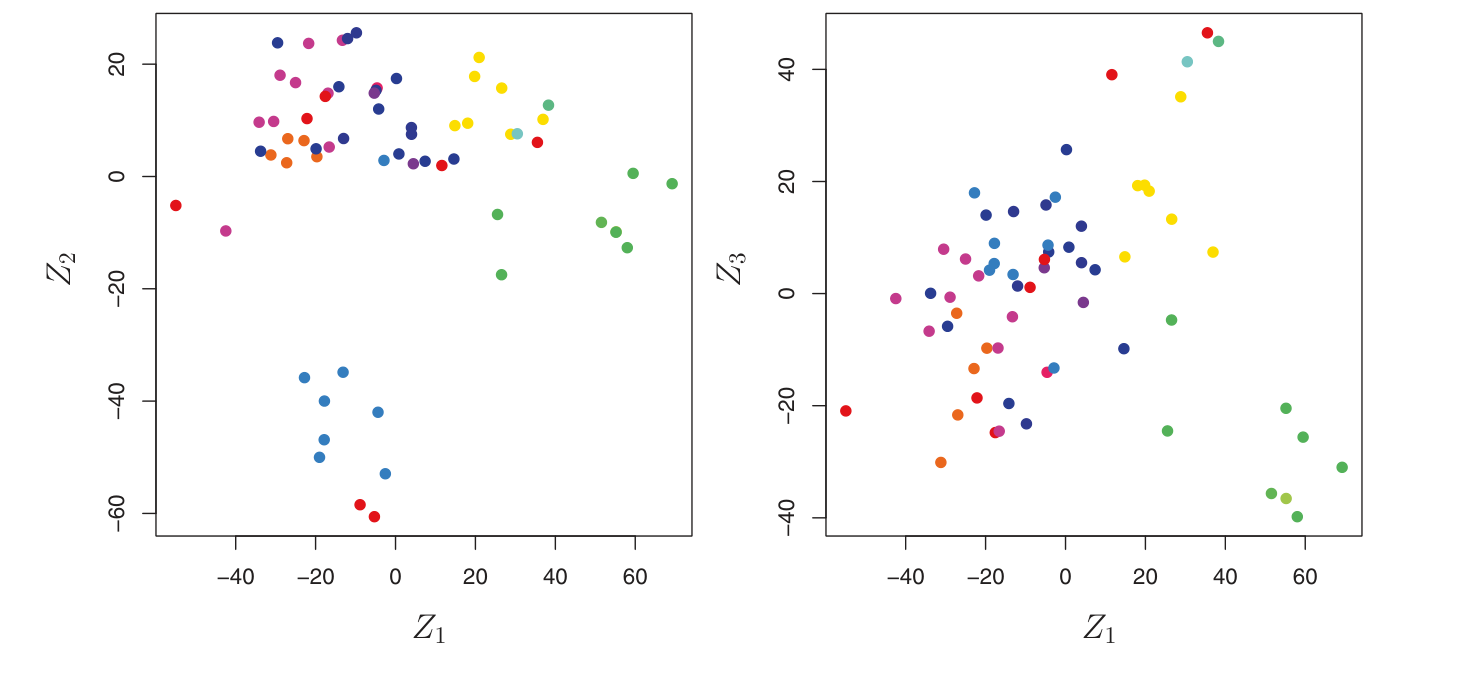
\includegraphics[width=0.65\textwidth]{../book/_static/book_figures/islr_fig10_15_nci60_pca.png}
  \end{center}
  \fuente{James, Witten, Hastie \& Tibshirani (2013), \textit{An Introduction to Statistical Learning}, Fig. 10.15.}
\end{frame}

\begin{frame}{\textit{Manifold learning}: el Swiss roll}
  \footnotesize
  PCA (lineal) colapsaría puntos lejanos en la superficie enrollada; el \textit{manifold learning} ``desenrolla'' la superficie preservando las distancias locales.
  \begin{center}
    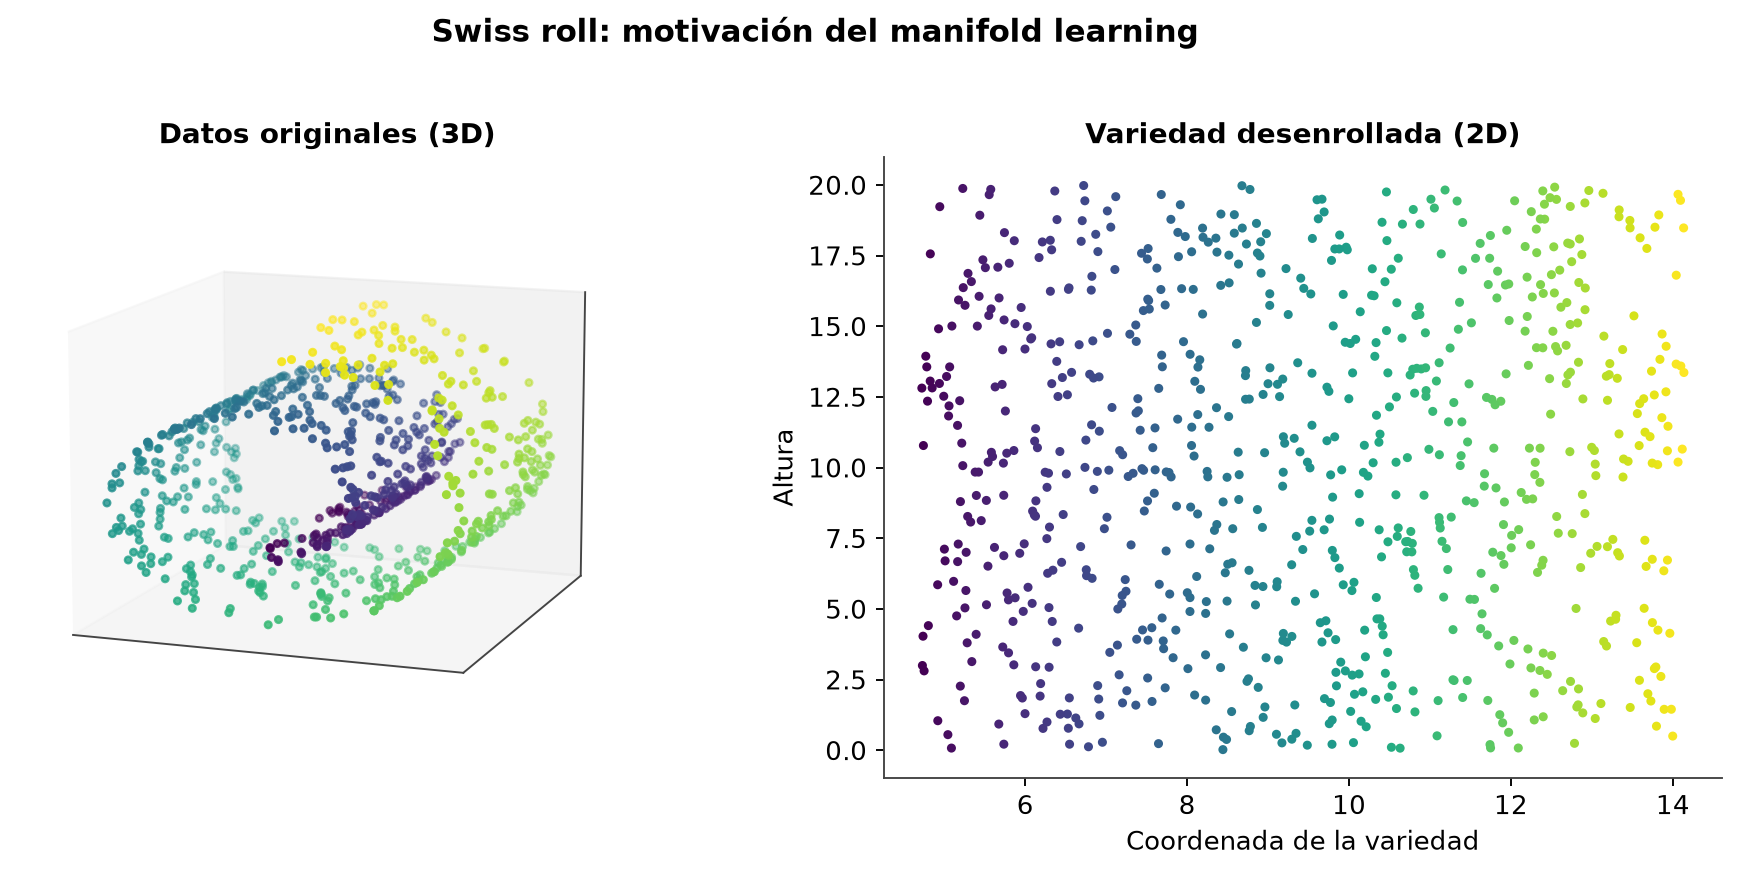
\includegraphics[width=0.85\textwidth]{../book/_static/generated/figures/es/swiss_roll_manifold.png}
  \end{center}
\end{frame}

\begin{frame}{t-SNE y UMAP}
  \begin{itemize}
    \item \textbf{t-SNE}: preserva vecindades locales; excelente para visualización, lento en datasets grandes
    \item \textbf{UMAP}: más rápido, preserva mejor la estructura global
    \item Ambos son no lineales — capturan relaciones que PCA no puede
  \end{itemize}
\end{frame}

\subsection{3.3 Detección de anomalías}

\begin{frame}{Filosofía de la detección de anomalías}
  \begin{itemize}
    \item \textit{Inliers} (normales) vs. \textit{outliers} (anomalías)
    \item \textbf{Anomaly detection}: dataset de entrenamiento contaminado
    \item \textbf{Novelty detection}: dataset de entrenamiento limpio
  \end{itemize}
\end{frame}

\begin{frame}{Enfoque gaussiano}
  \begin{itemize}
    \item Ajusta una distribución gaussiana (multivariante) a los datos normales
    \item Los puntos con baja densidad de probabilidad se marcan como anomalías
  \end{itemize}
  \begin{center}
    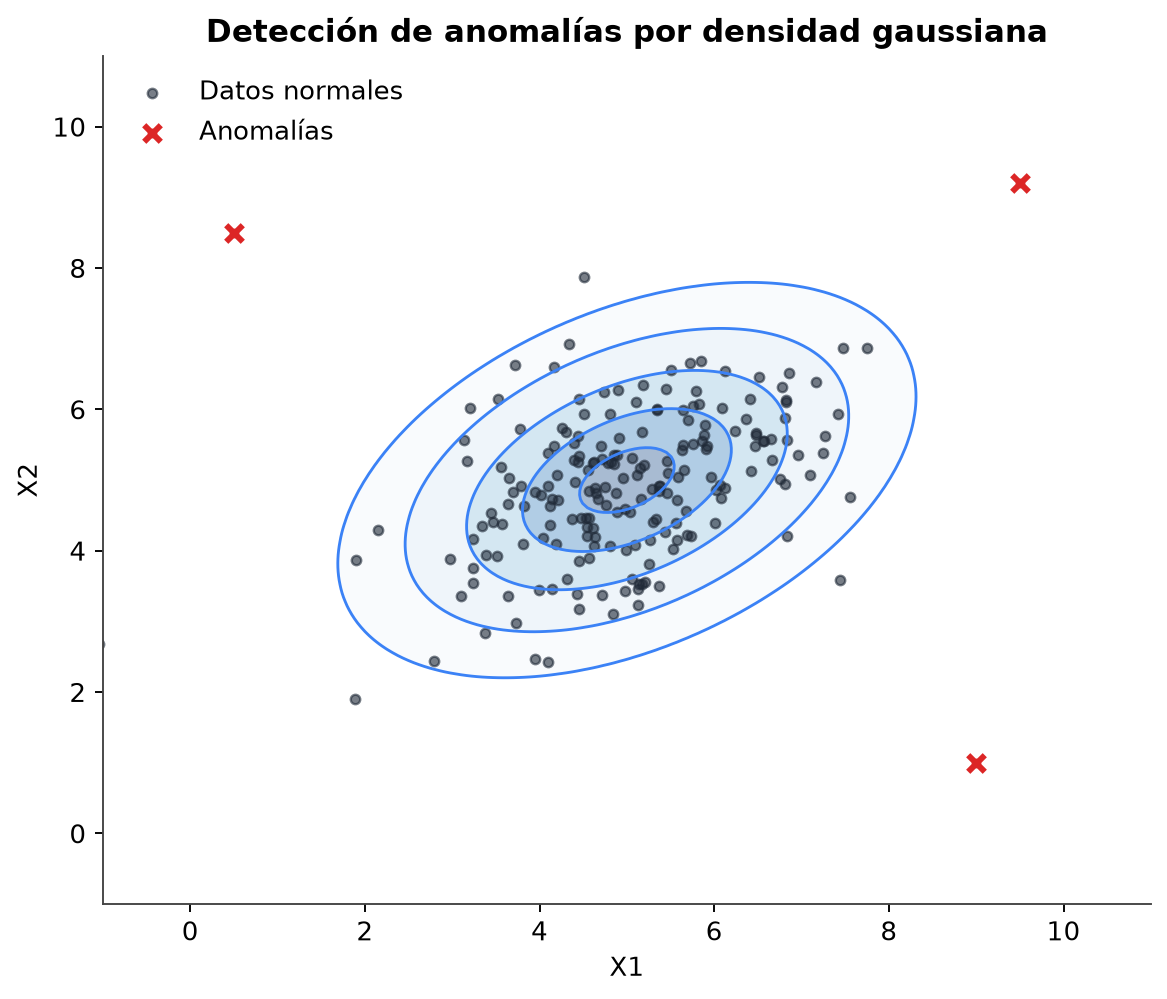
\includegraphics[width=0.42\textwidth]{../book/_static/generated/figures/es/gaussian_anomaly_detection.png}
  \end{center}
\end{frame}

\begin{frame}{Isolation Forest}
  \footnotesize
  Aísla puntos mediante particiones aleatorias del espacio de \textit{features}: las anomalías requieren muy pocas particiones para quedar aisladas.
  \begin{center}
    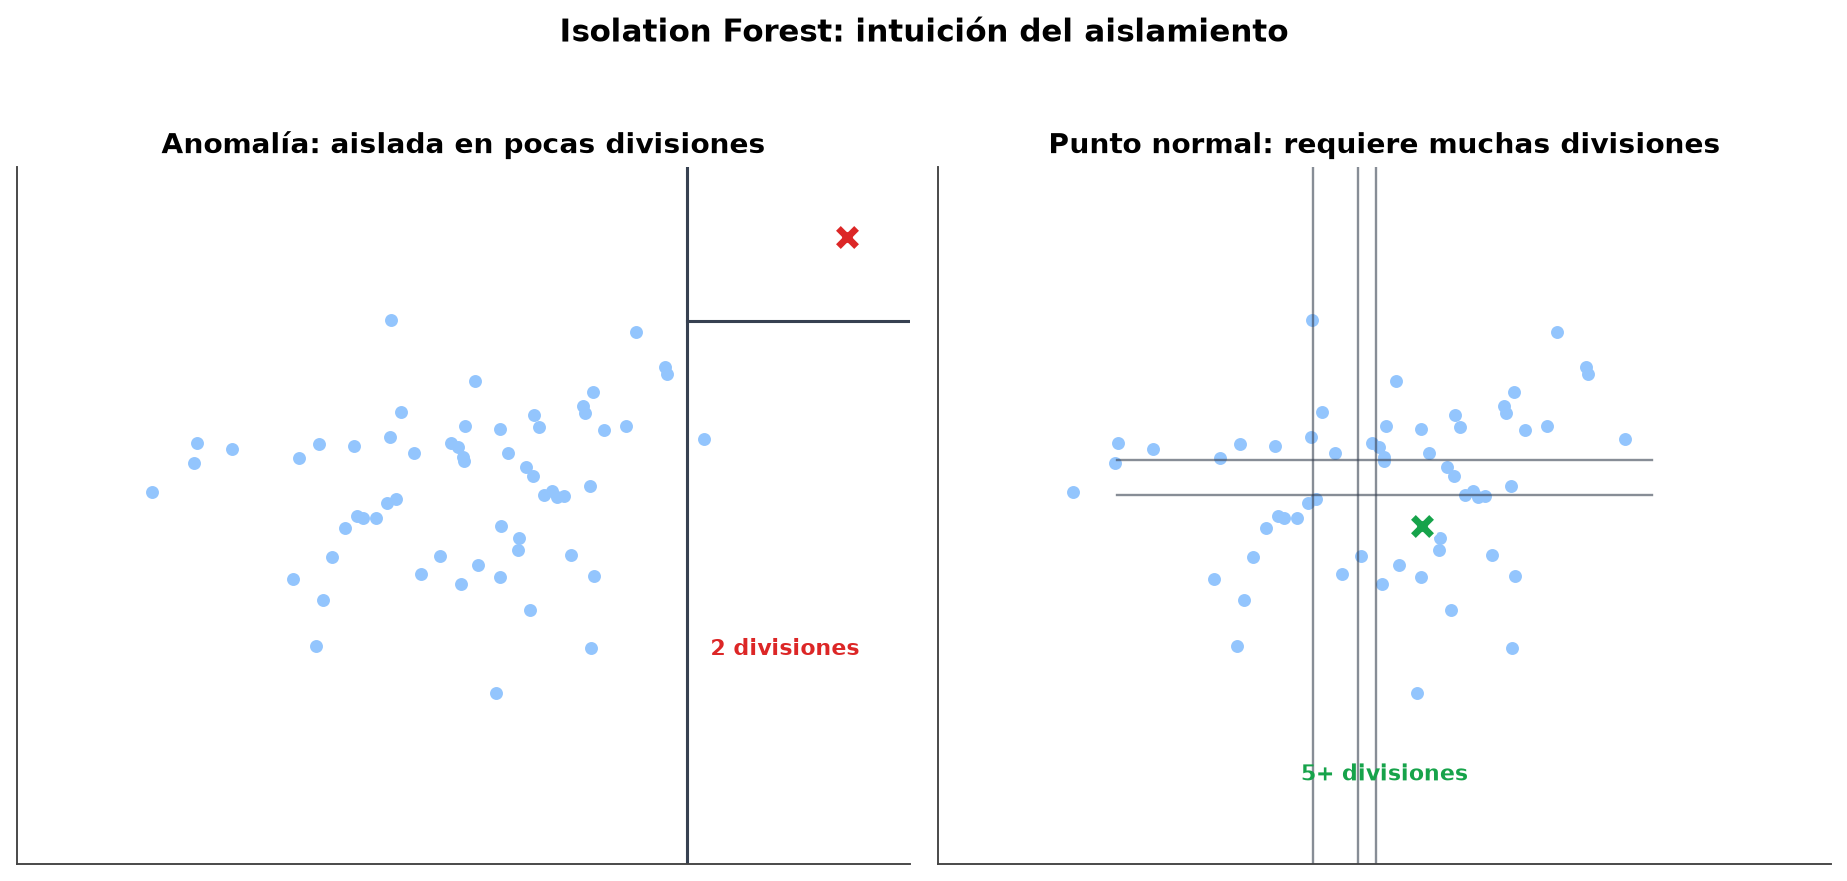
\includegraphics[width=0.85\textwidth]{../book/_static/generated/figures/es/isolation_forest_concept.png}
  \end{center}
\end{frame}

\begin{frame}{Local Outlier Factor (LOF)}
  \begin{itemize}
    \item Compara la densidad local de un punto con la de sus vecinos
    \item Detecta anomalías locales que un umbral de densidad global pasaría por alto
  \end{itemize}
  \begin{center}
    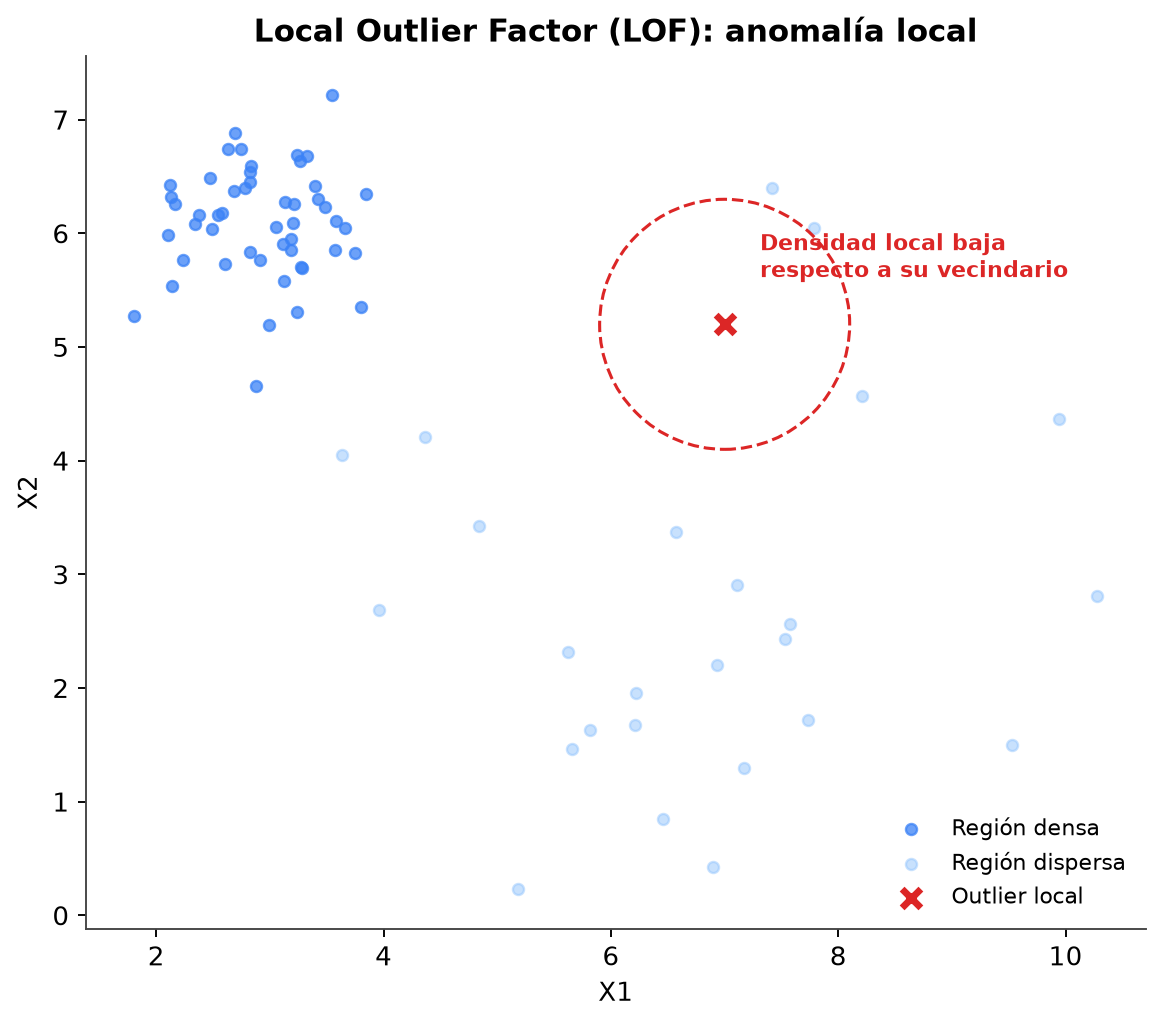
\includegraphics[width=0.42\textwidth]{../book/_static/generated/figures/es/lof_concept.png}
  \end{center}
\end{frame}

% ============================================================
\begin{frame}{Resumen del curso}
  \begin{columns}
    \begin{column}{0.33\textwidth}
      \textbf{Fundamentos}
      \begin{itemize}
        \footnotesize
        \item Historia del ML
        \item Overfitting/underfitting
        \item Validación cruzada
      \end{itemize}
    \end{column}
    \begin{column}{0.33\textwidth}
      \textbf{Supervisado}
      \begin{itemize}
        \footnotesize
        \item Regresión, regularización
        \item Clasificación, SVM
        \item Redes neuronales
      \end{itemize}
    \end{column}
    \begin{column}{0.33\textwidth}
      \textbf{No supervisado}
      \begin{itemize}
        \footnotesize
        \item Clustering
        \item PCA, manifold learning
        \item Detección de anomalías
      \end{itemize}
    \end{column}
  \end{columns}
\end{frame}

\begin{frame}
  \centering
  {\Huge ¡Gracias!}\\[1em]
  {\large Universidad de Salamanca}
\end{frame}

\end{document}
